\documentclass[a4paper, 10pt]{article}

\usepackage{amsmath}
\usepackage{amssymb}
\usepackage{cite}
\usepackage{color}
	\definecolor{gray}{rgb}{0.5,0.5,0.5}
\usepackage{colortbl}
\usepackage{datetime}
\usepackage{fancyvrb}
\usepackage{graphicx}
	\graphicspath{{images/}}
	\DeclareGraphicsExtensions{.eps, .pdf,.png}
\usepackage{epstopdf}
	\DeclareGraphicsRule{.eps}{pdf}{.pdf}{`epstopdf #1}
	\pdfcompresslevel=9
\usepackage{latexsym}
\usepackage[latin1]{inputenc}
\usepackage{listings}
	\lstset{
		frame=single,
		numbers=left,
		numberstyle=\small\color{gray},
		tabsize=4,
		morekeywords={and, boolean, do, else, false, for, if, integer, mod, true, until, wait, while},
	}
\usepackage{multirow}
\usepackage{relsize} % used for larger sum symbols
\usepackage{setspace}
%\usepackage{silence}% Filter out unwanted warnings and error messages
%\WarningFilter{pdftex}{destination with the same}
\usepackage{tikz}
	\usetikzlibrary{shapes, arrows, positioning}
	\tikzstyle{-}    = [draw]
	\tikzstyle{->}   = [draw, -latex']
	\tikzstyle{<-}   = [draw, latex'-]
	\tikzstyle{<->}  = [draw, latex'-latex']
	\tikzstyle{o}    = [draw, circle]
	\tikzstyle{box}  = [draw, rectangle]
\usepackage{url}

\usepackage{hyperref} % should be last usepackage to avoid errors.

\def \todo{\textbf{\textcolor{yellow}{TODO}}}
\def \citationneeded{\textbf{\textcolor{yellow}{CITATION NEEDED}}}
\newcommand{\listingrule}[1]{\rule{#1}{0.4pt}}

%\setcounter{secnumdepth}{5}

\title{Development and Analysis of Barrier Protocols}
\author{Ronny Brendel\\Tutors: Sascha Kl\"uppelholz \& Marcus V\"olp}

\begin{document}
%%%%%%%%%%%%%%%%%%%%%%%%%%%%%%%%%%%%%%%%%%%%%%%%%%%%%%%%%%%%%%%%%%%%%%%%%%%%%%%
\begin{titlepage}
\pagenumbering{alph}

\begin{center}
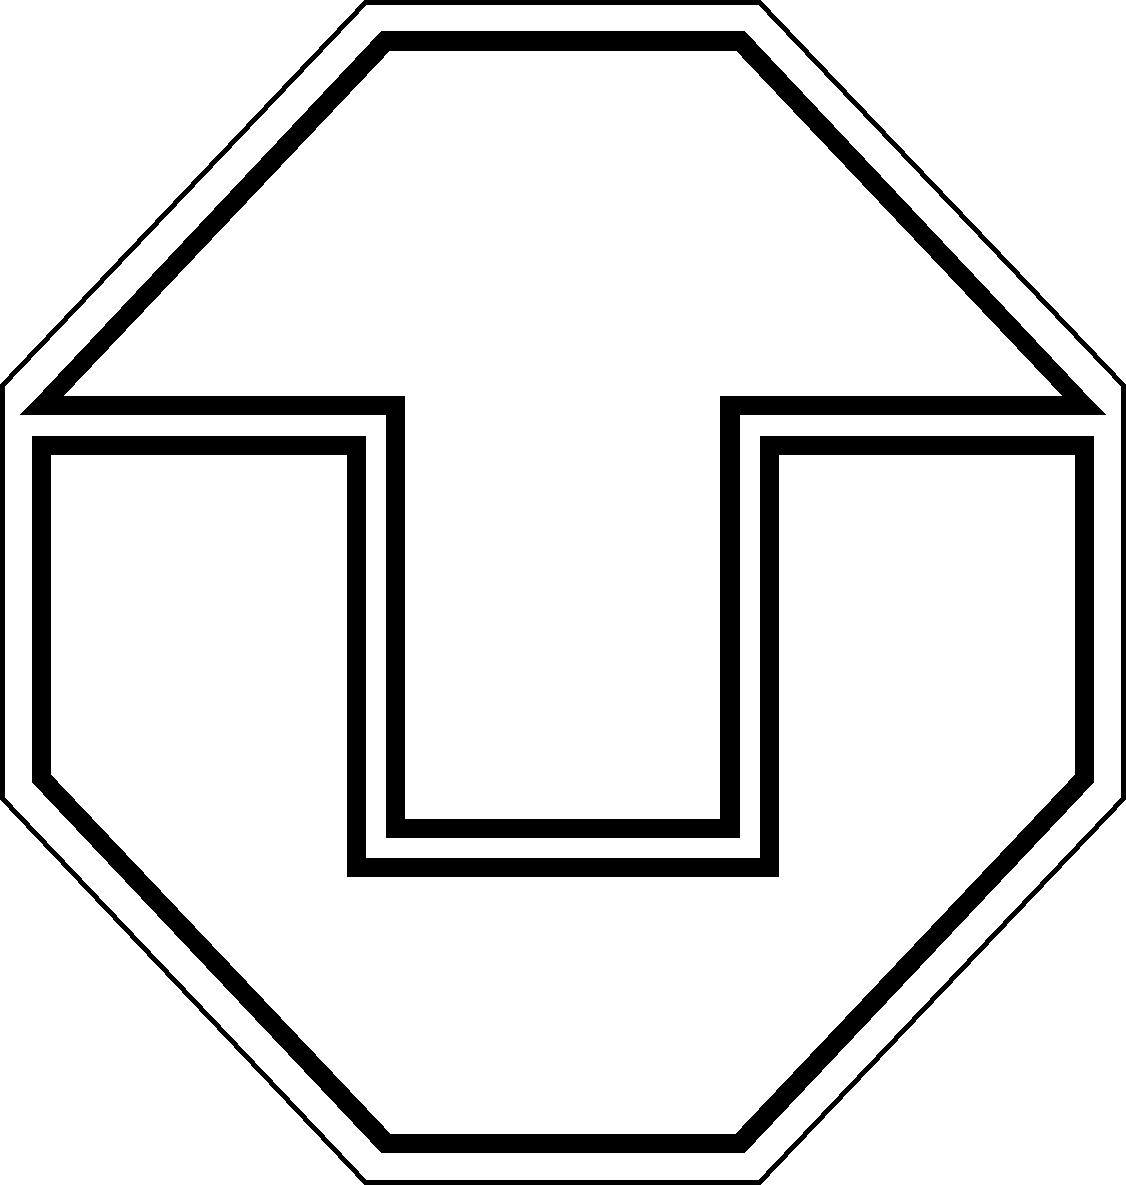
\includegraphics[width=3cm]{tu-logo}~\\[1cm]
\textsc{\LARGE Dresden University of Technology}\\[0.5cm]
\textsc{\Large Faculty of Computer Science}\\[0.2cm]
\textsc{\large Institute of Theoretical Computer Science}\\[0.2cm]
\textsc{\large Chair for Algebraic and Logical Foundations of Computer Science}\\[3cm]
\Huge Study's Thesis \\[1cm]
\huge Development and Analysis of Barrier Protocols\\[3cm]
\end{center}

\begin{flushleft} \large
	Author: Ronny Brendel \\
	Responsible university professor: Christel Baier \\
	Supervisors: Sascha Kl\"uppelholz \& Marcus V\"olp
\end{flushleft}

\vfill
\begin{flushright}
	\large October 2013
\end{flushright}

\end{titlepage}

\pagebreak
\newpage \thispagestyle{empty} \mbox{}
\pagebreak

%%%%%%%%%%%%%%%%%%%%%%%%%%%%%%%%%%%%%%%%%%%%%%%%%%%%%%%%%%%%%%%%%%%%%%%%%%%%%%%
\thispagestyle{empty}

%\section*{Aufgabenstellung}
%\label{sec:task}
%\begin{enumerate}
%	\item Literaturrecherche und ausf\"uhrlicher \"Uberblick aktuell genutzter Barrierenprotokolle sowie grunds\"atzlicher Implementierungsm\"oglichkeiten f\"ur Barrieren.
%	\item Untersuchung und Weiterentwicklung der von Nicolas Mc~Guire vorgeschlagenen Barriere.
%	\item Identifikation und Formalisierung der zentralen funktionalen Eigenschaften im Bezug auf Korrektheit sowie der quantitativen Eigenschaften zur Ermittlung der Performance von Barrierenprotokollen bez\"uglich Energieverbrauch und Geschwindigkeit.
%		\item Modellierung und Quantitative Analyse:
%			\begin{itemize}
%				\item Modellierung a) eines prominenten Vertreters von Barrierenprotokollen mit verteiltem Speicher, b) eines prominenten Vertreters von Barrierenprotokollen mit geteilten Speicher, c) des auf Mc~Guire beruhenden Barriereprotokolls jeweils im probabilistischem Model Checker PRISM.
%				\item Analyse und Vergleich der drei oben genannten Modelle im Bezug auf die in 3. identifizierten funktionalen sowie quantitativen Eigenschaften in PRISM. Wenn m\"oglich: Erg\"anzung des Performance-Vergleichs der drei Barrieren mittels messbasierter Methoden.
%			\end{itemize}
%		\item Zusammenfassung und Ausblick: Diskussion der in 4. gewonnenen Erkenntnisse
%\end{enumerate}
%
\section*{Task}
\label{sec:task}
\begin{enumerate}
	\item Literature research and detailed survey of currently used barrier protocols as well as implementation possibilities for barriers.
	\item Analysis and improvement of Nicolas Mc~Guire's proposed barrier.
	\item Identification and formalisation of key functional properties concerning correctness as well as quantitative aspects for determining performance of barrier protocols with regard to energy consumption and speed.
		\item Modelling and quantitative analysis:
			\begin{itemize}
				\item Modelling a) a prominent representative of barrier protocols for distributed memory, b) a prominent representative of barrier protocols for shared memory, c) the barrier protocol based on Mc~Guire's idea in each case using the probabilistic model checker PRISM.
				\item Analysis and comparison of the three above-mentioned models, regarding the functional as well as quantitative properties identified in 3., using PRISM. If possible: complement the performance evaluation of the three barriers using measurement-based methods.
			\end{itemize}
		\item Summary and outlook: Discussion of the insights gained in 4.
\end{enumerate}

\pagebreak
\newpage \thispagestyle{empty} \mbox{}
\pagebreak

%%%%%%%%%%%%%%%%%%%%%%%%%%%%%%%%%%%%%%%%%%%%%%%%%%%%%%%%%%%%%%%%%%%%%%%%%%%%%%%
\thispagestyle{empty}

%\section*{Selbstst\"andigkeitserkl\"arung}
%\label{sec:integrity}
%Ich erkl\"are hiermit, dass ich die vorliegende Arbeit selbst\"andig und ohne Benutzung anderer als der angegebenen Hilfsmittel angefertigt habe. Die aus fremden Quellen w\"ortlich oder sinngem\"a\ss ~\"ubernommenen Gedanken sind als solche kenntlich gemacht. Ich erkl\"are ferner, dass ich die vorliegende Arbeit an keiner anderen Stelle als Pr\"ufungsarbeit eingereicht habe oder einreichen werde.

\section*{Statement of academic integrity}
\label{sec:integrity}
I hereby declare that I prepared this thesis independently and without use of tools other than specified. Foreign thoughts, taken literally or in spirit, are marked as such. I also declare that I have not filed the present work at any other location or will submit it.

\pagebreak
\newpage \thispagestyle{empty} \mbox{}
\pagebreak

%%%%%%%%%%%%%%%%%%%%%%%%%%%%%%%%%%%%%%%%%%%%%%%%%%%%%%%%%%%%%%%%%%%%%%%%%%%%%%%
\thispagestyle{empty}

\renewcommand{\contentsname}{Table of contents}
\tableofcontents

\pagebreak
\newpage \thispagestyle{empty} \mbox{}
\pagebreak

%%%%%%%%%%%%%%%%%%%%%%%%%%%%%%%%%%%%%%%%%%%%%%%%%%%%%%%%%%%%%%%%%%%%%%%%%%%%%%%
\pagenumbering{arabic}
\section{Don't forget}
\begin{itemize}
	\item present tense! Consistency please! Exception where it makes sense.
	\item maybe increase font size in charts
	\item "don't overuse passive voice"
	\item be very aware where you use thread and process, and make sure the reader understands when the distinction does not matter
	\item make clear what is meant in the listings
		\begin{itemize}
			\item C-esque pseudo-code
			\item threadCount/processCount,  threadIndex/processIndex
			\item the code in the figures is executed on each thread. Each thread has an identifier between 0 and threadCount-1
			\item \& bit-wise \texttt{AND}, $|$ bit-wise \texttt{OR}, $\sim$ bit-wise \texttt{NOT}
			\item \texttt{x[$*$] := y} is short for assigning y to each element in x
			\item ?more?
		\end{itemize}
	\item mention that we assume atomic read and write at 32/64 bits a piece, when it matters
	\item explain cores vs processes, threads - we always assume threads, processes $>$= cores. Why. Find an appropriate spot to talk about this. I have marked a good spot in the text in Section~\ref{sssec:background-currently-used-shared}
	\item "be forthright about the limitations and assumptions of your design. Also, make sure you justify any shortcuts/limitations convincingly"
	\item \texttt{me} vs \texttt{threadIndex} / \texttt{processIndex}, make its use coherent
	\item color use in diagrams should be consistent (same bars should have same color across multiple diagrams)
	\item put raw data of figures into the appendix
\end{itemize}

%%%%%%%%%%%%%%%%%%%%%%%%%%%%%%%%%%%%%%%%%%%%%%%%%%%%%%%%%%%%%%%%%%%%%%%%%%%%%%%
\section{Introduction}
\label{sec:introduction}
\begin{itemize}
	\item \todo watch out that the intention/laying down a continuous thread is strong enough ((1)barriers can be improved, (2)through pW/CS, (3)model checking is useful)
	\item what is a barrier
	\item usage example for barriers
	\item barriers are common in parallel programming. OpenMP's\cite{openmp} implicit barriers. MPI barriers (Rolf Rabenseifner\cite{rab00}). Relate to normal send/recv, because absolute numbers without relation are not helpful.
		\begin{itemize}
			\item HLRS, year 2000
			\item many calls,
			\item 5.3\% of all time spent inside MPI calls, 0.7\% of all CPU time, estimated 1.6\% of the barrier execution time is actual synchronization, 100\% minus 1.6\% is waiting for other processes to arrive, because of unbalanced computation. Average 1852 microsecond per call. (Figure~13 in paper)
			\item e.g. receive 12.9\% of all time spent inside MPI calls, 1.8\% of all cpu time, 33\% of the recv executation time is actual latency plus transfer time, 100\% minus 33\% is waiting for other processes to arrive, because of unbalanced comoputation. Average 498 microseconds per call.
		\end{itemize}
	\item motivation for researching barriers: Apply ideas of pW/CS\cite{pwcs} to other synchronization primitives, e.g. barriers in order to gain performance, where performance can be any important measure e.g. speed, energy efficiency, (say something about possible improvements that can still be made).
	\item summarize pW/CS
		\begin{itemize}
			\item usually concurrent programs work in a deterministic fashion. That is the order and partners of remote synchronization (locally, programs are obviously mostly deterministic) are predetermined. The algorithm is executed in a very controlled fashion. Same holds for synchronization primitives themselves. Faulty behavior is avoided at great cost.
			\item don't avoid inconsistency at all cost. Make errors detectable, or ignorable.
			\item use the inherent randomness\cite{mcg09}, induced by caching, scheduling, randomness (ECC, flash access e.g.) at hardware level (jitter), or short: complexity of today's computer systems, in order to view concurrent accesses as really random. Thus we are able to apply probabilistic algorithms and analyse these algorithms using tools of probability theory.
			\item design algorithms that have sufficiently high probability of success and tolerate faulty behaviour.
			\item build them so that on average, or in their intended use case, they perform better than their deterministic counterparts, where better might e.g. be faster, more energy efficient, resource preserving.
			\item It seems to be a promising approach
			\item barriers can be improved. One possible way is through pW/CS.
		\end{itemize}
	\item how do we gather data on these algorithms to build confidence that they work properly, i.e. satisfy certain properties? And get a feeling for how they perform?
	\item Testing/Measurement (explain wording. Be aware of possible confusion) and model checking complement one another:
		\begin{itemize}
			\item Measurement is usually deterministic. If so, certain interesting states in a protocol are impossible to reach because of the randomness inherent to today's computers (add a short example? A special very case of a low level lock being contented?)
			\item Assuming you have randomized measurements, the probability to reach certain states in the protocol is so low that they are not revealed.
			\item Some parts of algorithms are performed in such a short time or need very exact preparation that it is practically impossible to analyse these parts using measurement. In this case model checking can be applied because it offers this granularity.
			\item Modelling has of course its own short comings. For example the state explosion problem.
			\item we can gain better quantitative insights into synchronization protocols by combining both measurement and model checking.
		\end{itemize}
	\item briefly explain the report structure
		\begin{itemize}
			\item existing stuff
				\begin{itemize}
					\item means to implement barriers
					\item currently used barriers
					\item idea to split barriers into orthogonal parts and think about them separately
				\end{itemize}
			\item new barriers
			\item analysis and comparison of one old for shared memory and one old for distributed memory against the new barriers
			\item conclusion \& future work
		\end{itemize}
\end{itemize}

%%%%%%%%%%%%%%%%%%%%%%%%%%%%%%%%%%%%%%%%%%%%%%%%%%%%%%%%%%%%%%%%%%%%%%%%%%%%%%%
\section{Background}
\label{sec:background}
In this section we will first take look at the tools at our disposal to implement barriers on both shared memory and distributed memory architectures.
Next we will show which barrier algorithms are used in today's parallel programming frameworks.
Finally we present a view of the barrier as a modularized algorithm consisting of various independent pieces.

%%%%%%%%%%%%%%%%%%%%%%%%%%%%%%%%%%%%%%%
\subsection{Means to implement barrier protocols}
\label{ssec:background-means}
A shared memory system consists of a number of processors which are connected to one chunk of memory they all share. Information can be exchanged between processors by simply writing and reading from same memory address, since they all share one address space.
Desktops, laptops and small to medium servers are typical examples of shared memory systems.

Many shared memory systems (called nodes) can be connected via a network to compose a distributed memory system. These systems do not have a global memory, instead each of the nodes has its own private memory. Computation is done locally on each node using only local memory. In order to share information between nodes the network messages need to be exchanged.
For example large servers and high-performance computers are oftentimes a distributed memory system.

Programming for shared memory and distributed memory architectures is very different. Thus we will subsequently differentiate between these two worlds.

%%%%%%%%%%%%%%%%%%%%
\subsubsection{Shared memory systems}
\label{sssec:background-means-shared}
A parallel program for on a shared memory system consists of multiple threads of execution -- short \emph{threads}.

The straightforward way to share a piece of information between threads is to \emph{load}, \emph{store} data from and to the same address.

Furthermore most modern processors provide means to execute a small series of computation on one date while making the memory unavailable to other threads. They are called \emph{atomic operations}. Two examples are the \emph{test-and-set} and \emph{add-fetch} instruction. The former stores a value to an address if a given condition is fulfilled, the latter loads a date, adds to it and stores it back.

Without these operations parallel programming is much more difficult and error-prone, since normal load and store can easily cause \emph{race conditions}. This convenience, on the other hand, comes at the cost of additional management overhead for the processor. To date cache coherent shared memory systems are usually limited to 64 threads and less. Some high-performance computing implementations reach numbers of 512 threads. In comparison distributed memory systems can have over a million threads.

The intuitive way memory access concurrently is \emph{sequentially consistent}.
\begin{quote}
	\textit{The result of any execution is the same as if the operations of all the processors were executed in some sequential order, and the operations of each individual processor appear in this sequence in the order specified by its program.} (Lamport~\cite{sequentialconsistency})
\end{quote}

Enforcing this intuitive semantic comes at a cost. Modern processors buffer memory access on many levels. To enforce sequential consistency mechanisms to control and circumvent this buffering have to be introduced resulting in more transistors in the processor and higher memory access latency.

If an algorithm is carefully designed, one can weaken the consistency model to gain better performance. One prominent way of such a model is \textit{release consistency}~\cite{gha90}. Memory accesses appears unordered except for so \emph{release} and \emph{acquire} operations. No memory access that has been issued after an acquire operation is permitted to finish before this acquire operation. No memory access is allowed to finish later than the next release operation. Acquire and release encapsulate the memory accesses in between.

Aside from implementing barriers in software vendors can wire barrier protocols into the system's hardware. This is almost never done on shared memory systems. One example for hardware barrier support is the SGI\textregistered UV\texttrademark 2000~\cite{sgiuv2000}, a high-performance shared memory computer.

%%%%%%%%%%%%%%%%%%%%
\subsubsection{Distributed memory systems}
\label{sssec:background-means-distributed}
A parallel program for a distributed memory architecture consists of multiple \emph{processes}. Each process has its own address space and is therefore unable to share memory with other processes.

First we will give an overview of general ways to implement synchronization primitives on distributed systems. Second we will have a look at one prominent distributed memory programming standard.

One way to exchange information between two processors is via \emph{synchronous message passing}. Two or more processors meet at a point in time until all communicating peers arrived, information is exchanged, and last all processes part and continue their computational tasks. This method requires all involved peers to shake hands. Information is buffered, queued and sent via network.

Another way to approach this is to wait as few as possible, since there is, for example, no need for a sending entity to wait until a receiver arrives. The sender might as well give his information to the communication framework and continue its computational work. This method is called \emph{asynchronous message passing}. Aside from less waiting time, asynchronous message passing incurs a similar overhead as synchronous message passing, because on the communication frame level similar work has to be done. Network channels have to be established, data has to be buffered and hands between peers have to be shaken.

A comparatively recent development is the move to \emph{remote memory access} (RMA). Remote memory access makes a portion of memory available via network so that others can load, store from and to it without actively involving the remote memory's owning processes. It is therefore sometimes called \emph{one-sided communication}. Implementations of RMA oftentimes support atomic operations.
In order for RMA to be available, the network hardware has to support it. For example InfiniBand~\cite{infiniband} has RMA facilities built in.

Hardware support for remote memory access is widespread especially in high-performance computing. Examples include the Earth Simulator~\cite{earthsimulator}, IBM Blue Gene/L~\cite{bluegenel}, IBM Blue Gene/Q~\cite{bluegeneq} and a low-cost custom system~\cite{hoefler2006b}

Another interesting and seemingly untested approach is to use lossy communication channels for developing synchronization protocols. Hardware is always erroneous -- for example conflicting network packages, dropped packages, corrupted packages or dropped connections happen all the time. To eliminate these errors protocols like the Transmission Control Protocol (TCP) are used amongst other techniques. Reliable protocols such as TCP incur a big performance penalty for transmitting short messages, since the packet size is huge in comparison to the data, each package has to be acknowledged by the receiver and other error checking facilities penalise latency further.
If one would instead craft algorithms so that it doesn't require a 100\% reliable connection, further performance improvements are conceivable.
Two ways such algorithms can be the implemented is via the User Datagram Protocol (UDP)~\cite{udp} and InfiniBand's unreliable connections~\cite{infiniband}.

\label{why-only-mpi}
We will now investigate the facilities the Message Passing Interface (MPI)~\cite{mpi3}, the most prominent high-performance distributed programming interface, provides us to implement barrier protocols. MPI is a standardised, low-level, language-independent and portable interface specification. It is very customizable and supports various modes of operation in order to support many different hardware configurations and allow the user to achieve maximum performance. MPI is widely adopted in high-performance computing (HPC) and scientific computing\cite{mpiadoptiona, mpiadoptionb, mpiadoptionc} and there exists a variety of implementations in all major programming languages.

In our analysis we will only scratch the surface of what the standard offers, since diving deep involves lots of details, complicated semantics and many of the details don't matter for our purpose.

MPI supports synchronous message passing via \emph{send} and \emph{receive}. Additionally you can issue a send operation that immediately returns if no receiver is already in place waiting for the sender.

Furthermore MPI facilitates asynchronous message passing. One can send and receive messages without blocking and one can test if a message has been successfully transmitted. Synchronous and asynchronous message passing can be mixed. That means one is able to, for example, issue a non-blocking send that is matched by a blocking receive operation.

Since version 3.0 the MPI standard supports \emph{non-blocking collectives}. Collectives is a collective name for all communication operations where there is a variable number of communicating  peers, like barrier, broadcast, reduce and more.
Non-blocking collectives allow, in the example of the barrier, to not block at the operation but to register at the barrier upon arrival, and subsequently test the barrier for completion while doing computational work in the meantime.
This facility is probably not suited to build new barriers on top of it, but is nevertheless an interesting development.

MPI also supports RMA. Although some MPI implementations, for example Open~MPI~\cite{openmpi}, do not support version 3.0 of the specification, we will restrict ourselves to analysing it, because it subsumes the features of version 2.2, it is already a year old and supported by other prominent implementations such as MPICH~\cite{mpich} 3.0 and derivatives like MVAPICH2\cite{mvapich} and Cray MPT\cite{craympt}.

The definition of RMA according to the standard is pretty involved, and we have to go into a bit more detail now to highlight important points. (mittelguter satz)

To initiate sharing remote memory each participating process issues a collective call to create a \emph{window} of memory to be shared. A window is associated with the group of processes that created it, and through it each participating process exposes a window of local memory to the other peers so they are able to access it in the future.
Upon creating a window a number of restrictions regarding the use of the window can be established in order to gain better performance. One can for example lower the memory consistency requirements or guarantee to not use certain operations.

Depending on the underlying hardware and the MPI implementation there are two different memory models. A window may either have the \emph{separate} or the \emph{unified} model. The separate model states that the copy of the remote memory that is visible to the remote peers and the copy that is visible to the local process is not the same and might therefore not automatically update between these two. That means a change by a peer to one process's memory might not be made visible. This process has to manually update its local copy. In contrast the unified model makes sure that the two copies are eventually updated. Therefore no manual update is necessary. This differentiation is a direct result of trying to support many different hardware configurations. With the upcoming standard 3.1 the user will be able to specify a minimum needed memory model. For now one can only ask the implementation which model is used.

Before going into the details of window synchronisation we have to introduce the concept of \emph{epochs}. An epoch is a period between two window synchronization calls. RMA operations like \emph{put}, \emph{get}, \emph{accumulate} may only be used inside an epoch. Epochs are used to accumulate multiple operations to one larger transfer in order to achieve better efficiency.

MPI differentiates between \emph{active} and \emph{passive} target communication. Active target communication involves both peers being actively involved in windows synchronization, whereas in passive target communication only one side's activity is required.

One way to synchronize a window is via a \emph{fence} operation. A fence is a collective operation among all window group members that makes sure that all outstanding RMA requests on this window are finished before the operation returns. It implies a full barrier synchronization.
A more fine-grained instance of active target communication is via the operations \emph{start}, \emph{complete}, \emph{post} and \emph{wait}. Before issuing any remote access calls the issuing process first has to advertise his intention through the start operation. Once he is finished he will invoke the complete operation to advertise that his transmission is done. The receiving end similarly issues post and wait to expose and synchronise its memory. The command receiving process may still access his window's local memory in the meantime. In contrast to a fence operation one can restrict such a synchronization to arbitrary processes of the window.

\begin{itemize}
	\item Don't use any MPI specific names. Keep it high-level
	\item MPI has RMA
		\begin{itemize}
			\item window sync
				\begin{itemize}
					\item MPI\_WIN\_LOCK, MPI\_WIN\_UNLOCK: Passive target communication. No explicit participation of remote peer in synchronization
					\item MPI\_Flush*: Passive target communication. Completes outstanding RMA calls, issued by the caller, at origin and a specifiable target before returning (or only at the origin).
					\item MPI\_Sync: Passive target communication. Used to synchronize the public and private part of the window in the separated model.
				\end{itemize}
			\item window sync assertions: NoPrecede, NoSucceed, NoStore, NoPut -$\>$ optimization
			\item MPI\_Put, MPI\_Get - unordered inside an epoch
			\item MPI\_Accumulate, MPI\_FetchAndOp, MPI\_CompareAndSwap influenced by specified memory order requirements. default is sequential consistency.
			\item list cases of undefined(implementation specific) behaviour: chapter 11.3 and 11.7 in \cite{mpi3}
				\begin{itemize}
					\item Buffers used in a MPI\_Put call should not be written to until the operation completes
					\item Buffers used in a MPI\_Get call should not be accessed until the operation completes
					\item The outcome of remote memory accesses to the same location is undefined. Except of course accumulate.
					\item concurrent local load/stores and RMA updates to the same location are undefined
					\item the outcome of a single process issuing multiple puts to the same location within an access epoch is undefined
					\item State that this makes it very hard to implement less restrictive synchronization primitives because the semantic requirements are already very strong in MPI. Lots of perhaps useless synchronization. Rather than undefined say: any order. Or at least make guarantee for the smallest units that are atomically committed to memory like primitive data types.
					\item perhaps state that in the following we will not implement, nor measure the performance of distributed memory algorithms. We will only measure shared memory stuff. But the will of course model check all the things.
				\end{itemize}
		\end{itemize}
\end{itemize}

\begin{itemize}
	\item most shared memory barriers rely on atomic operations
	\item most distributed memory barriers use synchronous message passing. These protocols have been implemented using RMA to improve efficeny, but they still behave exactly as if it was synchronous communication.
	\item as we will see in the next section
\end{itemize}

%%%%%%%%%%%%%%%%%%%%%%%%%%%%%%%%%%%%%%%
\subsection{Currently used barrier protocols}
\label{ssec:background-currently-used}

%%%%%%%%%%%%%%%%%%%%
\subsubsection{Shared memory systems}
\label{sssec:background-currently-used-shared}
\begin{itemize}
	\item explain short why only research in glibc and gnu openmp\cite{openmp}. closed source intel, microsoft, portland pgi, pathscale. pthreads und openmp open source und weit verbreitet. ?llvm?
	\item gnu openmp\cite{gomp}
		\begin{itemize}
			\item gcc 4.8.0, linux
			% gnu-openmp/gcc-4.8.0/libgomp/libgomp.h
			% gnu-openmp/gcc-4.8.0/libgomp/barrier.c
			% gnu-openmp/gcc-4.8.0/libgomp/config/linux/
			% gnu-openmp/gcc-4.8.0/libgomp/config/linux/bar.h
			% gnu-openmp/gcc-4.8.0/libgomp/config/linux/bar.c
			% gnu-openmp/gcc-4.8.0/libgomp/config/linux/futex.h (cpu_relax)
			% gnu-openmp/gcc-4.8.0/libgomp/config/linux/wait.h
			\item Central Counter Barrier with atomic add and fetch
			\item Figure~\ref{fig:pseudo-code-central-counter}
				\begin{figure}[htbp]
					\centering
					\begin{minipage}
\centering
\begin{lstlisting}[mathescape, linewidth=10.4cm]
shared variables: integer barrier := threadCount
$\listingrule{10.4cm}$

atomic{barrier := barrier - 1}

wait until barrier = 0
\end{lstlisting}
\end{minipage}

					\caption{Pseudo code of the Central Counter Barrier}
					\label{fig:pseudo-code-central-counter}
				\end{figure}
			\item Figure~\ref{fig:diagram-central-counter}
				\begin{figure}[htbp]
					\centering
					%\begin{tikzpicture}[node distance = 2.0cm, auto]
\begin{tikzpicture}[]

\node [draw=none]        (a)  {Atomic decrement:};
\node [o,   below of=a]  (0a) {0};
\node [o,   right of=0a] (1a) {1};
\node [o,   right of=1a] (2a) {2};
\node [o,   right of=2a] (3a) {3};
\node [o,   right of=3a] (4a) {4};
\node [box, below of=2a] (Va) {barrier};

\path [<->] (0a) edge (Va)
            (1a) edge (Va)
            (2a) edge (Va)
            (3a) edge (Va)
            (4a) edge (Va);

\node [draw=none, below of=0a]     (middle) {};

\node [draw=none, below of=middle] (b)      {Repeatedly read:};
\node [o,   below of=b]            (0b)     {0};
\node [o,   right of=0b]           (1b)     {1};
\node [o,   right of=1b]           (2b)     {2};
\node [o,   right of=2b]           (3b)     {3};
\node [o,   right of=3b]           (4b)     {4};
\node [box, below of=2b]           (Vb)     {barrier};

\path [->] (Vb) edge (0b)
           (Vb) edge (1b)
           (Vb) edge (2b)
           (Vb) edge (3b)
           (Vb) edge (4b);

\end{tikzpicture}

					\caption{The two phases of the Central Counter Barrier}
					\label{fig:diagram-central-counter}
				\end{figure}
			\item explain algorithm in detail here
			\item is in reality more complex. For example back-off via a spin-counter $\sim$ 3ms. architecture specific. futexes\cite{franke2002}. kernel based mutexes. wait queues. sleeping. lowers spincount if core count $<$ thread count.
			\item talk about us assuming core count $>$= thread count. (from don't forget)
			\item reset built in. Last one to enter resets the barrier.
		\end{itemize}
	\item glibc's\cite{glibc} new pthreads library
		\begin{itemize}
			\item version 2.17. is in my ubuntu raring 13.04.
			% glibc/nptl/sysdeps/pthread/pthread.h
			% glibc/nptl/pthread_barrier_*
			% glibc/nptl/sysdeps/unix/sysv/linux/internaltypes.h
			\item Central Counter with locking instead of atomic add-fetch
			\item back-off through futexes (without spinning before)
			\item reset handled automatically (upon leaving the barrier every thread increments (atomically) the barrier by 1 so that it is max in the end)
		\end{itemize}
\end{itemize}

%%%%%%%%%%%%%%%%%%%%
\subsubsection{Distributed memory systems}
\label{sssec:background-currently-used-distributed}
\begin{itemize}
	\item only MPI implementations. Why has already been explained in Section~\ref{why-only-mpi}.
	\item only openmpi and mpich. Explain why. (opensource. mpich is base of many others (name them). weit verbreitete implementationen.)
	\item openmpi
		\begin{itemize}
			\item version 1.7. not yet released.
			% ompi/mca/coll/tuned/coll_tuned_barrier.c :
			% ompi_coll_tuned_barrier_intra_recursivedoubling,
			% ompi_coll_tuned_barrier_intra_bruck
			% ompi/mca/coll/tuned/coll_tuned_decision_fixed.c
			\item $n \neq 2^k \rightarrow$ Dissemination\cite{hensgen1988} using sync sendrecv
			\item $n = 2^k \rightarrow$ recursive doubling (explanation e.g. in \cite{hoefler2005})
			\item back-off hard to determine. probably through OPAL\_THREAD\_(UN)LOCK in the end
			\item resetting (in both algorithms) not necessary since sendrecv sets up itself newly everytime.
			\item architecture specific for infiband. e.g. Dissemination using RMA \cite{hoefler2006a}
			\item state that we use an RMA representation of the algorithm. Maybe state why. Writing is sending. Reading is Receiving so to speak.
			\item Figure~\ref{fig:pseudo-code-dissemination}
				\begin{figure}[htbp]
					\centering
					\begin{center}
\begin{minipage}{\textwidth}
\begin{lstlisting}[mathescape, linewidth=11.2cm]
constants:        me := processIndex
shared variables: boolean
                  barrier[processCount][processCount]
local variables:  integer dist, to, from
initialisation:   barrier[*][*] := false
$\listingrule{11.2cm}$

dist := 1
while dist < processCount {
	to   := (me + dist) (mod processCount)
	from := (me - dist) (mod processCount)
	
	barrier[to][me] := true
	
	wait until barrier[me][from] = true

	dist := dist $\cdot$ 2
}
\end{lstlisting}
\end{minipage}
\end{center}

					\caption{Pseudo code of the Dissemination Barrier}
					\label{fig:pseudo-code-dissemination}
				\end{figure}
			\item Figure~\ref{fig:diagram-dissemination}
				\begin{figure}[htbp]
					\centering
					%\begin{tikzpicture}[node distance = 2.0cm, auto]
\begin{tikzpicture}[]

%pivotal nodes
\node [draw=none                 ]   (a) {Round 1:};
\node [o, below of=a             ]  (0a) {0};
\node [below of=0a, draw=none    ]   (b) {Round 2:};
\node [o, below of=b             ]  (0b) {0};
\node [below of=0b, draw=none    ]   (c) {Round 3:};
\node [o, below of=c             ]  (0c) {0};

\clip (-0.5cm,0) rectangle (7.5cm,-6cm);

% round 1
\node [   left of=0a , draw=none ] (07a);
\node [o, right of=0a            ]  (1a) {1};
\node [o, right of=1a            ]  (2a) {2};
\node [o, right of=2a            ]  (3a) {3};
\node [o, right of=3a            ]  (4a) {4};
\node [o, right of=4a            ]  (5a) {5};
\node [o, right of=5a            ]  (6a) {6};
\node [o, right of=6a            ]  (7a) {7};
\node [o, right of=7a, draw=none ] (70a);

\path [->] (07a) edge [distance=0.2cm]  (0a)
            (0a) edge [distance=0.2cm]  (1a)
            (1a) edge [distance=0.2cm]  (2a)
            (2a) edge [distance=0.2cm]  (3a)
            (3a) edge [distance=0.2cm]  (4a)
            (4a) edge [distance=0.2cm]  (5a)
            (5a) edge [distance=0.2cm]  (6a)
            (6a) edge [distance=0.2cm]  (7a);
\path [-]   (7a) edge [distance=0.2cm] (70a);

% round 2
\node [   left of=0b , draw=none ] (07b);
\node [   left of=07b, draw=none ] (06b);
\node [o, right of=0b            ]  (1b) {1};
\node [o, right of=1b            ]  (2b) {2};
\node [o, right of=2b            ]  (3b) {3};
\node [o, right of=3b            ]  (4b) {4};
\node [o, right of=4b            ]  (5b) {5};
\node [o, right of=5b            ]  (6b) {6};
\node [o, right of=6b            ]  (7b) {7};
\node [o, right of=7b, draw=none ] (70b);
\node [o, right of=70b, draw=none] (71b);

\path [->] (06b) edge [distance=0.6cm]                 (0b)
           (07b) edge [distance=0.6cm,out=-45,in=225]  (1b)
            (0b) edge [distance=0.6cm]                 (2b)
            (1b) edge [distance=0.6cm,out=-45,in=225]  (3b)
            (2b) edge [distance=0.6cm]                 (4b)
            (3b) edge [distance=0.6cm,out=-45,in=225]  (5b)
            (4b) edge [distance=0.6cm]                 (6b)
            (5b) edge [distance=0.6cm,out=-45,in=225]  (7b);
\path [-]   (6b) edge [distance=0.6cm]                (70b)
            (7b) edge [distance=0.6cm,out=-45,in=225] (71b);

%round 3
\node [   left of=0c , draw=none ] (07c);
\node [   left of=07c, draw=none ] (06c);
\node [   left of=06c, draw=none ] (05c);
\node [   left of=05c, draw=none ] (04c);
\node [o, right of=0c            ]  (1c) {1};
\node [o, right of=1c            ]  (2c) {2};
\node [o, right of=2c            ]  (3c) {3};
\node [o, right of=3c            ]  (4c) {4};
\node [o, right of=4c            ]  (5c) {5};
\node [o, right of=5c            ]  (6c) {6};
\node [o, right of=6c            ]  (7c) {7};
\node [   right of=7c , draw=none] (70c);
\node [   right of=70c, draw=none] (71c);
\node [   right of=71c, draw=none] (72c);
\node [   right of=72c, draw=none] (73c);

\path [->] (04c) edge [distance=0.8cm]  (0c)
           (05c) edge [distance=0.8cm,out=-45,in=225]  (1c)
           (06c) edge [distance=0.8cm]  (2c)
           (07c) edge [distance=0.8cm,out=-45,in=225]  (3c)
            (0c) edge [distance=0.8cm]  (4c)
            (1c) edge [distance=0.8cm,out=-45,in=225]  (5c)
            (2c) edge [distance=0.8cm]  (6c)
            (3c) edge [distance=0.8cm,out=-45,in=225]  (7c);
\path [-]   (4c) edge [distance=0.8cm] (70c)
            (5c) edge [distance=0.8cm,out=-45,in=225] (71c)
            (6c) edge [distance=0.8cm] (72c)
            (7c) edge [distance=0.8cm,out=-45,in=225] (73c);

\end{tikzpicture}

					\caption{The rounds of the Dissemination Barrier}
					\label{fig:diagram-dissemination}
				\end{figure}
			\item explain algorithm in detail here
			\item things to explain
				\begin{itemize}
					\item each array (first index) is located on the respective process's memory
				\end{itemize}

		\end{itemize}
	\item mpich
		\begin{itemize}
			\item many mpi implementations are based on mpich (e.g. mvapich2, intel mpi, cray mpi,
			\item many can not be inspected because source is closed
			\item version 3.0.4. current today
			% src/mpi/coll/barrier.c : MPIR_Barrier_intra
			\item log2 Dissemination with sendrecv. same as openmpi
		\end{itemize}
	\item Dissemination can also be used for shared memory\cite{hoefler2013}
\end{itemize}

%%%%%%%%%%%%%%%%%%%%%%%%%%%%%%%%%%%%%%%
\subsection{Barrier building blocks}
\label{ssec:building-blocks}
\begin{itemize}
	\item latency/computation trade-off
	\item resetting:
		\begin{itemize}
			\item how is resetting handled in currently used barriers?
			\item integrated in the barrier ``self-resetting''
			\item use 3 barriers reset barrier x+2 when you finished barrier x. switch between the barriers by checking if barrier x+2 is reset or not (as in central-counter-with-reset). Describe in pseudo code as well, maybe.
			\item if variable space permits it you can also change the variables to 'counters' and modify all checks to ask for numbers modulo round + a check that you are in the proper round
		\end{itemize}
	\item back-off
	\item thread count $<$= cores, thread count $>$ cores
	\item combining: we can combine barrier protocols. Explain how. Reap benefits, mitigate shortcomings. Adapt to topology (explain. Node shared mem, internode dist mem., different interconnect topologies) aware.
\end{itemize}

%%%%%%%%%%%%%%%%%%%%%%%%%%%%%%%%%%%%%%%%%%%%%%%%%%%%%%%%%%%%%%%%%%%%%%%%%%%%%%%
\section{Three new barriers}
\label{sec:new}
\begin{itemize}
	\item put some introductory text here
	\item \todo pay attention where to draw the line between this section and the analysis in the next section (perhaps, leave some/most of the analysis for the next section)
	\item \todo elegantly transition to Ronny's fancy barrier (distributed memory case). Suddenly talking about processes and remote/local memory is bad.
\end{itemize}
%%%%%%%%%%%%%%%%%%%%%%%%%%%%%%%%%%%%%%%
\subsection{Mc~Guire/Ronny barrier}
\label{ssec:new-nmg}
\begin{itemize}
	\item original idea by Nicholas Mc Guire was given to me in a private communique.
	\item modification of the original protocol resulted in Figure~\ref{fig:pseudo-code-nmg-ronny}
	\item first appearance in \cite{bre13}. Slight modification since then "remembers others" considered here. Don't explain in detail what the modification is and does, since the reader has no knowledge of the previous version and I don't want to explain all of it.
		\begin{figure}[htbp]
			\centering
			\begin{center}
\begin{minipage}{\textwidth}
\begin{lstlisting}[mathescape, linewidth=11.4cm]
constants:        meBit:=$2^\mathit{threadIndex}$, full:=$\sum_{i=0}^{\mathit{threadCount}-1}2^i$
local variables:  integer copy
shared variables: integer entry, exit, boolean left
initialisation:   entry := 0, exit := 0, left := false
$\listingrule{11.4cm}$

if left = false {

	do {
		copy := (copy $\&$ $\sim$meBit) | entry
		if copy $\&$ meBit = 0 {
			copy  := copy | meBit
			entry := copy
		}
	} while copy $\neq$ full and left = false

	left := true
	exit := 0

} else if left = true {

	do {
		copy := (copy $\&$ $\sim$meBit) | exit
		if copy $\&$ meBit = 0 {
			copy := copy | meBit
			exit := copy
		}
	} while copy $\neq$ full and left = true

	left  := false
	entry := 0
}
\end{lstlisting}
\end{minipage}
\end{center}

			\caption{Pseudo code of Mc Guire/Ronny's barrier}
			\label{fig:pseudo-code-nmg-ronny}
		\end{figure}
	\item high-level explanation
	\item detailed walk through one iteration
	\item advantage: no atomic ops
	\item resetting is integrated. Needs a little less space than the approaches shown in Section~\ref{ssec:building-blocks}
	\item Limited to 64 threads in this version. But one can modify the protocol to use an array of bit masks, representing a big bit mask. Updating the bit mask will then only be done on the element where the updating thread is itself located on. This way we only write one 64 bit value which is committed atomically. If we would attempt to write more than one element, we would run into consistency problems. Reading the shared variable will then read the whole array instead.
\end{itemize}

%%%%%%%%%%%%%%%%%%%%%%%%%%%%%%%%%%%%%%%
\subsection{Ronny's simple barrier}
\label{ssec:new-simple}
\begin{itemize}
	\item new and shiny. Read mostly, write exactly once. In contrast to Mc Guire/Ronny's barrier.
	\item How did I come up with the idea?
	\item Figure~\ref{fig:pseudo-code-ronny-simple}
		\begin{figure}[htbp]
			\centering
			\begin{center}
\begin{minipage}{\textwidth}
\begin{lstlisting}[mathescape, linewidth=9.7cm]
shared variables: boolean barrier[threadCount]
local variables:  integer i
initialization:   barrier[*] := false
$\listingrule{9.7cm}$

barrier[threadIndex] := true

i := 0
while i < threadCount {
	if barrier[i] = false {
		i := -1
	}
	i = i + 1
}
\end{lstlisting}
\end{minipage}
\end{center}

			\caption{Pseudo code of Ronny's simple barrier}
			\label{fig:pseudo-code-ronny-simple}
		\end{figure}
	\item explanation here.
	\item one array element per cache line to avoid false sharing\cite{falsesharing}
	\item every thread writes into the array element he owns. Indicated by his threadIndex.
	\item do not mention (analysis section instead): in contrast to the central-counter barrier the assignments to shared variables can be done in parallel, since the variables written are not the same, no are they on the same cache line.
	\item (do not mention. Is in the analysis) many read accesses, but since data is cached upon the first read the latency is only significant once per array element / cache line. i.e. when the thread arrives and writes his array element to be \texttt{true} and when a thread reads it after it has been written by it's owner.
	\item advantage: no atomic ops
	\item (do not mention. Is in the analysis) larger memory cost than Central Counter, Mc Guire/Ronny. They number of barriers per thread team should be 1 at most, thus the memory overhead is still negligible.
	\item The barrier is destructive in the sense that it cannot be executed multiple times in a row. One way to circumvent this is to modify the algorithm to use a repetition counter instead of a boolean (since we have one date per cache line we allocated the space anyways) and keep track of it. The algorithm would then atomically increase the counter instead of the assignment in line 4. We use a 64 bit integer variable for this. It will not overflow over so we don't need to consider this case (If you could run one barrier each clock cycle on a 3GHz machine you would need roughly 200 years to overflow it).
	\item another small improvement would be to keep track of the first couple of successfully read entries and skip those when repeating the loop. For simplicity's sake and modelling we will not consider this optimization.
\end{itemize}

%%%%%%%%%%%%%%%%%%%%%%%%%%%%%%%%%%%%%%%
\subsection{Ronny's fancy barrier}
\label{ssec:new-fancy}
\begin{itemize}
	\item variation of Ronny's simple barrier where not only will the own presence be stored, but the presence of other processes, we know have arrived, as well.
	\item evaluation has shown that cache latency is so low, that the additional computation this mechanism introduces, makes this algorithm run slower on shared memory systems than the unmodified one. Thus we will now switch to a distributed memory scenario where communication latency is much higher. If we assume RMA for communication we can use the protocol without modification.
	\item Figure~\ref{fig:pseudo-code-ronny-fancy}
		\begin{figure}[htbp]
			\centering
			\begin{center}
\begin{minipage}{\textwidth}
\begin{lstlisting}[mathescape, linewidth=11.5cm]
constants:        me := processIndex, meBit := $2^{me}$,
                  full := $\sum_{i=0}^{\mathit{processCount}-1}2^i$
shared variables: integer barrier[processCount]
local variables:  integer i
initialization:   barrier[*] := 0
                  i := processIndex
$\listingrule{11.5cm}$

barrier[me] := meBit;

do {
	do {
		i := i + 1 (mod processCount)
	} while barrier[me] $\&$ $2^i$ = 1

	barrier[me] := barrier[me] | barrier[i]
} while barrier[me] $\neq$ full
\end{lstlisting}
\end{minipage}
\end{center}

			\caption{Pseudo code of Ronny's fancy barrier}
			\label{fig:pseudo-code-ronny-fancy}
		\end{figure}
	\item each array element is located in the memory of the respective process.
	\item Only the own element is written. Only remote reading.
	\item When a process reads remotely he is informed of other processes, the remote peer knows, have arrived.
	\item probabilistic runtime. Depending on circumstances the protocol will finish in more or less steps (or perhaps successful non-zero reads). It is not predetermined what is communicated and with whom.
	\item advantage: no atomic ops. The writing does not have to be atomic, since processes only write to local memory, and no inconsistent data can be read since 64 bit reads and writes are atomic.
	\item more computational overhead (bit shuffling) for less communication.
	\item discuss resetting through triple barrier. Perhaps, briefly hint that this kind of resetting can be added to any barrier (perhaps add a listing how this would look like (the spin model should have it, or one of the pseudo code files)), more on this in the section on the orthogonal design of barriers.
	\item restricted to 64 threads. An extension to arrays of bit masks, similar to the Mc Guire/Ronny barrier is possible.
\end{itemize}

%%%%%%%%%%%%%%%%%%%%%%%%%%%%%%%%%%%%%%%%%%%%%%%%%%%%%%%%%%%%%%%%%%%%%%%%%%%%%%%
\section{Analysis and comparison}
\label{sec:analysis}
\begin{itemize}
	\item \todo maybe distinguish extreme cases vs more normal cases. And the spectrum in between -- adds structure -- is nice.
	\item In this section we will evaluate one commonly used barrier for each shared memory and distributed memory architectures and pit them against one novel protocol in each category.
	\item Early evaluations have shown the Mc Guire/Ronny's barrier to perform worse than the Central Counter Barrier, whereas Ronny's simple and fancy barrier show promise. Therefore we restrict our attention to the latter.
	\item For the shared memory case the Central Counter Barrier (Figure~\ref{fig:pseudo-code-central-counter} in Section~\ref{sssec:background-currently-used-shared}) is pitted against Ronny's simple barrier (Figure~\ref{fig:pseudo-code-ronny-simple} in Section~\ref{ssec:new-simple}).
	\item For distributed memory architectures the Dissemination Barrier (Figure~\ref{fig:pseudo-code-dissemination} in Section~\ref{sssec:background-currently-used-distributed}) and Ronny's fancy barrier (Figure~\ref{fig:pseudo-code-ronny-fancy} in Section~\ref{ssec:new-fancy}) are compared. (explain choice with a few words? -- ref existing-currently-used?)
	\item In our evaluations we always assume no back-off strategy is used. Each algorithm polls busily on the requested variable until the desired value is read. Threads do not wait sleeping or use callback mechanisms. The topic of back-off strategies is a large and intricate subject in its own right and goes beyond the scope of this thesis.
	\item The analysis is split into two parts: general properties (bla, perceived without measuring, bla), model checking.
\end{itemize}

%%%%%%%%%%%%%%%%%%%%%%%%%%%%%%%%%%%%%%%
\subsection{General properties}
\label{ssec:analysis-general}
\begin{itemize}
	\item group properties into measurable and non-measurable (model checking, sharp looking at)
	\item present considerations of interest about the chosen algorithms.
\end{itemize}

%%%%%%%%%%%%%%%%%%%%
\paragraph{Shared memory barriers}
\label{sssec:analysis-general-shared}
\begin{itemize}
	\item don't talk cache specifics, because we have not given an introduction to MSI. Express yourself in simple terms.
	\item ref algorithms
	\item make sure that people understand it is about shared read/write, not local variables.
	\item PHASES: both algorithms are performed in two phases. A writing phase and a reading phase.
	\item In the writing phase of the Central Counter Barrier concurrently issued add-fetch operations will be queued (because atomic ops on a single variable). On the other hand Ronny's simple barrier allocates one cache line per array element. Thus all writes to shared memory can be executed in parallel. If all threads arrive at the same instant, writing can be sped up to a factor of $\mathit{threadCount}$ in comparison to executing serialized write operations. In more balanced scenarios this effect diminishes.
	\item The reading phase of the Central Counter Barrier reads a single variable repeatedly. The cache line this variable resides on will be invalidated for each core exactly $\mathit{threadCount} - 1$ times (disregarding outside influences) ((, thus each core fetches the variable at most $\mathit{threadCount} - 1$ times)).
	\item The reading phase of Ronny's simple barrier needs to read each array element once until it can make a decision whether to leave or repeat the loop. Each array element is invalidated exactly once. Thus each array element, from the viewpoint of one thread, has to be fetched from memory at most twice. From then on it is cached and quickly accessible.
	\item the Central Counter Barrier has the obvious advantage in this phase. How big this advantage is depends heavily on the underlying hardware. For example if the cache line prefetcher predicts the access pattern of the reading phase of Ronny's simple barrier, those reads can be executed in parallel. (Vorsicht. Evtl weglassen)
	\item The Central Counter Barrier is quicker during busy waiting, whereas Ronny's simple barrier performs well during writing. We attempt to quantify the effects of this behaviour in the following subsections.
	\item MEMORY: the Central Counter barrier needs a logarithmic amount of memory in the number of threads (i.e. 64 bits, for up to $2^{64}$ threads), whereas Ronny's simple barrier needs a linear amount -- $\mathit{threadCount} \cdot 64$ bytes, assuming a cache line is 64 bytes. This looks like a lot, but since shared memory systems rarely exceed 512 cores, a maximum of only about 32KiB of memory would be used. 64 bytes per thread. Furthermore one thread team needs only one barrier and repeat it. There would be no benefit in allocating the memory for more than one.
\end{itemize}

%%%%%%%%%%%%%%%%%%%%
\paragraph{Distributed memory barriers}
\label{sssec:analysis-general-distributed}
\begin{itemize}
	\item ref algorithms
	\item For the Dissemination Barrier the number of remote writes is exactly $n \cdot \lceil \log _2~n \rceil$ -- $n$ processes times $\lceil \log _2~n \rceil$ rounds. Dissemination remotely writes more than the minimum needed in order to gain speed over the straightforward gather + broadcast approach, which is, illustrated in Figure~\ref{fig:diagram-gather-broadcast}, $2 \cdot (n-1)$ writes in $2 \cdot  \lceil \log _2~n \rceil$ rounds.
		\begin{figure}[htbp]
			\centering
			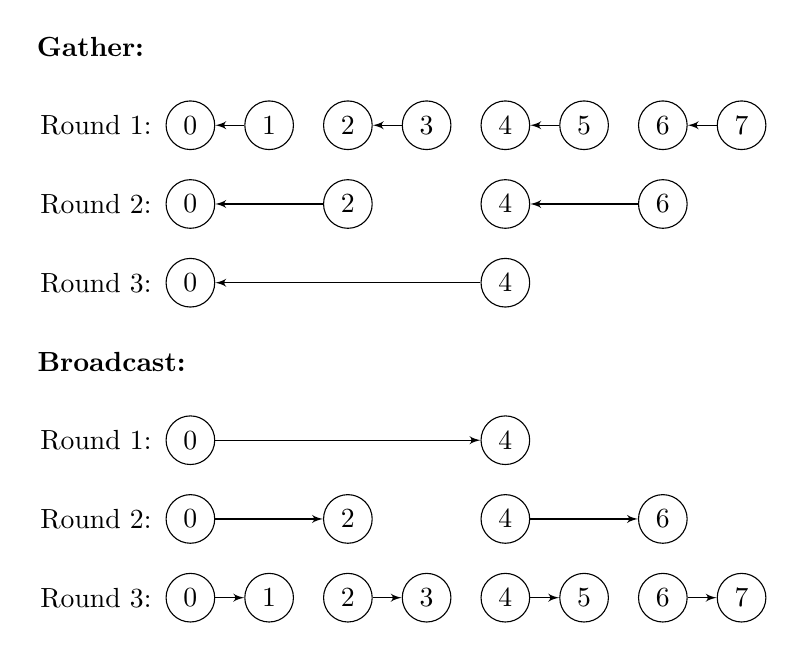
\begin{tikzpicture}[]

%pivotal nodes
\node [               draw=none  ]   (a) {};
\node [left of=a     ,draw=none,distance=2cm  ]  (ya) {\textbf{Gather:~~~~~}};
\node [o, below of=a,            ]  (0a) {0};
\node [o, below of=0a            ]  (0b) {0};
\node [o, below of=0b            ]  (0c) {0};
\node [below of=0c   , draw=none ]   (d) {};
\node [left of=d     , draw=none ]  (yd) {\textbf{Broadcast:}};
\node [o, below of=d             ]  (0d) {0};
\node [o, below of=0d            ]  (0e) {0};
\node [o, below of=0e            ]  (0f) {0};

% gather 1
\path (0a) ++(180:1.2cm) node []    (xa) {Round 1:};
\node [o, right of=0a            ]  (1a) {1};
\node [o, right of=1a            ]  (2a) {2};
\node [o, right of=2a            ]  (3a) {3};
\node [o, right of=3a            ]  (4a) {4};
\node [o, right of=4a            ]  (5a) {5};
\node [o, right of=5a            ]  (6a) {6};
\node [o, right of=6a            ]  (7a) {7};

\path [<-] (0a) edge (1a)
           (2a) edge (3a)
           (4a) edge (5a)
           (6a) edge (7a);

% gather 2
\path (0b) ++(180:1.2cm) node []    (xb) {Round 2:};
\node [o, right of=0b,draw=none  ]  (1b) {};
\node [o, right of=1b            ]  (2b) {2};
\node [o, right of=2b,draw=none  ]  (3b) {};
\node [o, right of=3b            ]  (4b) {4};
\node [o, right of=4b,draw=none  ]  (5b) {};
\node [o, right of=5b            ]  (6b) {6};
\node [o, right of=6b,draw=none  ]  (7b) {};

\path [<-] (0b) edge (2b)
           (4b) edge (6b);

% gather 3
\path (0c) ++(180:1.2cm) node []    (xc) {Round 3:};
\node [o, right of=0c,draw=none  ]  (1c) {};
\node [o, right of=1c,draw=none  ]  (2c) {};
\node [o, right of=2c,draw=none  ]  (3c) {};
\node [o, right of=3c            ]  (4c) {4};
\node [o, right of=4c,draw=none  ]  (5c) {};
\node [o, right of=5c,draw=none  ]  (6c) {};
\node [o, right of=6c,draw=none  ]  (7c) {};

\path [<-] (0c) edge (4c);

% broadcast 1
\path (0d) ++(180:1.2cm) node []    (xd) {Round 1:};
\node [o, right of=0d,draw=none  ]  (1d) {};
\node [o, right of=1d,draw=none  ]  (2d) {};
\node [o, right of=2d,draw=none  ]  (3d) {};
\node [o, right of=3d            ]  (4d) {4};
\node [o, right of=4d,draw=none  ]  (5d) {};
\node [o, right of=5d,draw=none  ]  (6d) {};
\node [o, right of=6d,draw=none  ]  (7d) {};

\path [->] (0d) edge (4d);

% broadcast 2
\path (0e) ++(180:1.2cm) node []    (xe) {Round 2:};
\node [o, right of=0e,draw=none  ]  (1e) {};
\node [o, right of=1e            ]  (2e) {2};
\node [o, right of=2e,draw=none  ]  (3e) {};
\node [o, right of=3e            ]  (4e) {4};
\node [o, right of=4e,draw=none  ]  (5e) {};
\node [o, right of=5e            ]  (6e) {6};
\node [o, right of=6e,draw=none  ]  (7e) {};

\path [->] (0e) edge (2e)
           (4e) edge (6e);

% broadcast 3
\path (0f) ++(180:1.2cm) node []    (xf) {Round 3:};
\node [o, right of=0f            ]  (1f) {1};
\node [o, right of=1f            ]  (2f) {2};
\node [o, right of=2f            ]  (3f) {3};
\node [o, right of=3f            ]  (4f) {4};
\node [o, right of=4f            ]  (5f) {5};
\node [o, right of=5f            ]  (6f) {6};
\node [o, right of=6f            ]  (7f) {7};

\path [->] (0f) edge (1f)
           (2f) edge (3f)
           (4f) edge (5f)
           (6f) edge (7f);

\end{tikzpicture}

			\caption{Communication pattern of a basic gather and broadcast barrier}
			\label{fig:diagram-gather-broadcast}
		\end{figure}

	\item Reading is only done locally.
	\item Ronny's fancy barrier needs between $2 \cdot (n-1)$ and $n \cdot (n-1)$ successful (non-zero) remote reads. Writing is only done locally. (perhaps add picture of n*(n-1), n*(n-1) might also be completely wrong)
	\item failed remote gets. Maybe give a rough estimate of the lost bandwidth.
	\item Dissemination needs exactly $\lceil \log _2~n \rceil$ rounds. Ronny's fancy barrier does not have rounds and tries reading from the next process regardless of whether a remote read has been successful (non-zero) where the Dissemination Barrier waits for its designated communication partner.
	\item needing $\lceil \log _2~n \rceil$ rounds is obviously worse than $\log _2~n$. This especially means that from $n$, where $n$ is a power of 2 threads, to $n+1$ number of rounds increases by 1. Therefore, for core counts other that are not a power of two, the performance degrades. Super wasteful shows a more balanced picture with increasing core counts where Dissemination has jumps at power of two core counts. Benchmarks on shared memory have shown this to be true.
	\item MEMORY: The memory requirements of the Dissemination Barrier and Ronny's fancy barrier are the same. Each process uses some local memory to keep track of the other processes. The exact number depends on the implementation. Theoretically $\lceil \log _2~n \rceil$ bits per process for both algorithms suffice. The Dissemination variant shown in Figure~\ref{fig:pseudo-code-dissemination} uses a total of $n \cdot n$ bits, but, since each thread communicates only with $\lceil \log _2~n \rceil$ other threads, a modified index calculation would allow it to work with $n \cdot \lceil \log _2 ~n \rceil$ bits. The memory usage is minuscule either way.
	\item the progress problem
		\begin{itemize}
			\item normal Figure~\ref{fig:diagram-dissemination} in Section~\ref{sssec:background-currently-used-distributed}. All processes arrive timely.
			\item more normal that one or more processes are missing.
			\item how much progress can a barrier make while not all processes have arrived?
			\item suppose process 4 has not entered. Modified diagram of the progress through the rounds: Figure~\ref{fig:diagram-dissemination-progress}
				\begin{figure}[htbp]
					\centering
					%\begin{tikzpicture}[node distance = 2.0cm, auto]
\begin{tikzpicture}[]

%pivotal nodes
\node [o, below of=xxx]  (0a) {0};
\path (0a) ++(-90:1.4cm) node [draw, circle, node] (0b) {0};
\path (0b) ++(-90:1.8cm) node [draw, circle, node] (0c) {0};

\path (0a) ++(180:1.4cm) node [node] (xa) {Round 1:};
\path (0b) ++(180:1.4cm) node [node] (xb) {Round 2:};
\path (0c) ++(180:1.4cm) node [node] (xc) {Round 3:};

\clip (-0.5cm,0) rectangle (7.5cm,-6cm);

% round 1
\node [   left of=0a , draw=none ] (07a) {};
\node [o, right of=0a            ]  (1a) {1};
\node [o, right of=1a            ]  (2a) {2};
\node [o, right of=2a            ]  (3a) {3};
\node [o, right of=3a, dotted    ]  (4a) {4};
\node [o, right of=4a            ]  (5a) {5};
\node [o, right of=5a            ]  (6a) {6};
\node [o, right of=6a            ]  (7a) {7};
\node [o, right of=7a, draw=none ] (70a) {};

\path [->] (07a) edge [distance=0.2cm        ]  (0a)
            (0a) edge [distance=0.2cm        ]  (1a)
            (1a) edge [distance=0.2cm        ]  (2a)
            (2a) edge [distance=0.2cm        ]  (3a)
            (3a) edge [distance=0.2cm        ]  (4a)
            (4a) edge [distance=0.2cm, dotted]  (5a)
            (5a) edge [distance=0.2cm        ]  (6a)
            (6a) edge [distance=0.2cm        ]  (7a);
\path [-]   (7a) edge [distance=0.2cm        ] (70a);

% round 2
\node [   left of=0b , draw=none ] (07b) {};
\node [   left of=07b, draw=none ] (06b) {};
\node [o, right of=0b            ]  (1b) {1};
\node [o, right of=1b            ]  (2b) {2};
\node [o, right of=2b            ]  (3b) {3};
\node [o, right of=3b, dotted    ]  (4b) {4};
\node [o, right of=4b, dotted    ]  (5b) {5};
\node [o, right of=5b            ]  (6b) {6};
\node [o, right of=6b            ]  (7b) {7};
\node [o, right of=7b, draw=none ] (70b) {};
\node [o, right of=70b, draw=none] (71b) {};

\path [->] (06b) edge [distance=0.6cm                       ]  (0b)
           (07b) edge [distance=0.6cm,out=-45,in=225        ]  (1b)
            (0b) edge [distance=0.6cm                       ]  (2b)
            (1b) edge [distance=0.6cm,out=-45,in=225        ]  (3b)
            (2b) edge [distance=0.6cm                       ]  (4b)
            (3b) edge [distance=0.6cm,out=-45,in=225        ]  (5b)
            (4b) edge [distance=0.6cm               , dotted]  (6b)
            (5b) edge [distance=0.6cm,out=-45,in=225, dotted]  (7b);
\path [-]   (6b) edge [distance=0.6cm                       ] (70b)
            (7b) edge [distance=0.6cm,out=-45,in=225        ] (71b);

%round 3
\node [   left of=0c , draw=none ] (07c) {};
\node [   left of=07c, draw=none ] (06c) {};
\node [   left of=06c, draw=none ] (05c) {};
\node [   left of=05c, draw=none ] (04c) {};
\node [o, right of=0c            ]  (1c) {1};
\node [o, right of=1c            ]  (2c) {2};
\node [o, right of=2c            ]  (3c) {3};
\node [o, right of=3c, dotted    ]  (4c) {4};
\node [o, right of=4c, dotted    ]  (5c) {5};
\node [o, right of=5c, dotted    ]  (6c) {6};
\node [o, right of=6c, dotted    ]  (7c) {7};
\node [   right of=7c , draw=none] (70c) {};
\node [   right of=70c, draw=none] (71c) {};
\node [   right of=71c, draw=none] (72c) {};
\node [   right of=72c, draw=none] (73c) {};

\path [->] (04c) edge [distance=0.8cm               , dotted]  (0c)
           (05c) edge [distance=0.8cm,out=-45,in=225, dotted]  (1c)
           (06c) edge [distance=0.8cm               , dotted]  (2c)
           (07c) edge [distance=0.8cm,out=-45,in=225, dotted]  (3c)
            (0c) edge [distance=0.8cm                       ]  (4c)
            (1c) edge [distance=0.8cm,out=-45,in=225        ]  (5c)
            (2c) edge [distance=0.8cm                       ]  (6c)
            (3c) edge [distance=0.8cm,out=-45,in=225        ]  (7c);
\path [-]   (4c) edge [distance=0.8cm               , dotted] (70c)
            (5c) edge [distance=0.8cm,out=-45,in=225, dotted] (71c)
            (6c) edge [distance=0.8cm               , dotted] (72c)
            (7c) edge [distance=0.8cm,out=-45,in=225, dotted] (73c);

\end{tikzpicture}

					\caption{Progression through the rounds of the Dissemination Barrier with process four not having entered}
					\label{fig:diagram-dissemination-progress}
				\end{figure}
			\item process 4 does not notify process 5, therefore in the next round process 5 cannot notify process 7 and so on.
			\item number of blocked processes doubles each round.
			\item once process 4 arrives each one of these blocked processes then needs to finish the still to do rounds until the protocol succeeds
			\item who knows of whose arrival Figure~\ref{tab:table-dissemination-progress}
				\begin{table}[htbp]
					\centering
					\caption{Which process knows of which other's arrival}
					\vspace{0.2cm}
					\begin{minipage}{0.42\linewidth}
						\textbf{After round 1:} \\
						$(n-1) + (n-1) = 14$ \\
						\vspace{-0.1cm} \\
						\resizebox{5cm}{!}{
							\begin{tabular}{c | c c c c c c c c}
								  & 0        & 1        & 2        & 3        & 4 & 5        & 6        & 7 \\
								\hline
								0 & $\times$ &          &          &          &         &          &          & $\times$ \\
								1 & $\times$ & $\times$ &          &          &         &          &          &          \\
								2 &          & $\times$ & $\times$ &          &         &          &          &          \\
								3 &          &          & $\times$ & $\times$ &         &          &          &          \\
								4 &          &          &          & $\times$ &         &          &          &          \\
								5 &          &          &          &          &         & $\times$ &          &          \\
								6 &          &          &          &          &         & $\times$ & $\times$ &          \\
								7 &          &          &          &          &         &          & $\times$ & $\times$ \\
							\end{tabular}
						}
					\end{minipage}
					\begin{minipage}{0.42\linewidth}
						\textbf{After round 2:} \\
						$14 + 6 \cdot 2 = 26$ \\
						\vspace{-0.1cm} \\
						\resizebox{5cm}{!}{
							\begin{tabular}{c | c c c c c c c c}
								  & 0        & 1        & 2        & 3        & 4 & 5        & 6        & 7 \\
								\hline
								0 & $\times$ &          &          &          &   & $\times$ & $\times$ & $\times$ \\
								1 & $\times$ & $\times$ &          &          &   &          & $\times$ & $\times$ \\
								2 & $\times$ & $\times$ & $\times$ &          &   &          &          & $\times$ \\
								3 & $\times$ & $\times$ & $\times$ & $\times$ &   &          &          &          \\
								4 &          & $\times$ & $\times$ & $\times$ &   &          &          &          \\
								5 &          &          & $\times$ & $\times$ &   & $\times$ &          &          \\
								6 &          &          &          &          &   & $\times$ & $\times$ &          \\
								7 &          &          &          &          &   &          & $\times$ & $\times$ \\
							\end{tabular}
						}
					\end{minipage}
					\begin{minipage}{0.42\linewidth}
						\vspace{0.3cm}
						\textbf{After round 3}: \\
						$26 + 4 \cdot 4 = 44$ \\
						\vspace{-0.1cm} \\
						\resizebox{5cm}{!}{
							\begin{tabular}{c | c c c c c c c c}
								  & 0        & 1        & 2        & 3        & 4 & 5        & 6        & 7 \\
								\hline
								0 & $\times$ &          &          &          &        & $\times$ & $\times$ & $\times$ \\
								1 & $\times$ & $\times$ &          &          &        &          & $\times$ & $\times$ \\
								2 & $\times$ & $\times$ & $\times$ &          &        &          &          & $\times$ \\
								3 & $\times$ & $\times$ & $\times$ & $\times$ &        &          &          &          \\
								4 & $\times$ & $\times$ & $\times$ & $\times$ &        & $\times$ & $\times$ & $\times$ \\
								5 & $\times$ & $\times$ & $\times$ & $\times$ &        & $\times$ & $\times$ & $\times$ \\
								6 & $\times$ & $\times$ & $\times$ &          &        & $\times$ & $\times$ & $\times$ \\
								7 & $\times$ & $\times$ & $\times$ & $\times$ &        &          & $\times$ & $\times$ \\
							\end{tabular}
						}
					\end{minipage}
					\begin{minipage}{0.42\linewidth}
						\vspace{0.3cm}
						\textbf{Ronny's fancy:} \\
						$(n-1) \cdot (n-1) = 49$ \\
						\vspace{-0.1cm} \\
						\resizebox{5cm}{!}{
							\begin{tabular}{c | c c c c c c c c}
								  & 0        & 1        & 2        & 3        & 4 & 5        & 6        & 7 \\
								\hline
								0 & $\times$ & $\times$ & $\times$ & $\times$ &   & $\times$ & $\times$ & $\times$ \\
								1 & $\times$ & $\times$ & $\times$ & $\times$ &   & $\times$ & $\times$ & $\times$ \\
								2 & $\times$ & $\times$ & $\times$ & $\times$ &   & $\times$ & $\times$ & $\times$ \\
								3 & $\times$ & $\times$ & $\times$ & $\times$ &   & $\times$ & $\times$ & $\times$ \\
								4 &          &          &          &          &   &          &          &          \\
								5 & $\times$ & $\times$ & $\times$ & $\times$ &   & $\times$ & $\times$ & $\times$ \\
								6 & $\times$ & $\times$ & $\times$ & $\times$ &   & $\times$ & $\times$ & $\times$ \\
								7 & $\times$ & $\times$ & $\times$ & $\times$ &   & $\times$ & $\times$ & $\times$ \\
							\end{tabular}
						}
					\end{minipage}
					\label{tab:table-dissemination-progress}
				\end{table}
			\item for non-power of two process counts the effect worsens. Where for power of two process counts $n-1$ remote writes need to be executed before the barrier is finished, non-power of two process counts need to issue $2^{\lceil \log_2 n \rceil} - 1$ writes.
			\item ronny's fancy does need multiple rounds to finish. The last arriving thread can fetch all others from one other process. And all others need to do one more successful remote read. Therefore $n$ remote reads, which can be issued in parallel, are needed to complete the barrier.
			\item quantifying this effect will be done in the following section.
		\end{itemize}
\end{itemize}

%%%%%%%%%%%%%%%%%%%%%%%%%%%%%%%%%%%%%%%
\subsection{Model checking}
\label{ssec:analysis-modelchecking}
\begin{itemize}
	\item SPIN\cite{spin, hol97}, PRISM\cite{prism, knp09}
\end{itemize}

%%%%%%%%%%%%%%%%%%%%
\subsubsection{Preliminaries}
\label{sssec:analysis-modelchecking-preliminaries}
\begin{itemize}
	\item continuous-time Markov chains.
	\item further details in textbooks like \cite{kul95, ks76}
	\item if $S$ is a finite set, then a distribution on $S$ is a function $\nu:S \rightarrow [0,1]$ with $\sum\limits_{s \in S} \nu (s) = 1$. For $U \subseteq S$, $\nu (U)$ is a shortform notation for $\sum\limits_{s \in U} \nu (s)$.
	\item CTMC tuple $\mathcal{M} = (S, \mathit{Act}, R, \mu)$, where $S$ is a finite set of states, $Act$ a finite set of action names and $R$ a function of type $S \times \mathit{Act} \times S \rightarrow \mathbb{R}_{\ge 0}$, called the rate matrix of $\mathcal{M}$. $\mu$ is a distribution on $S$ specifying the probabilities for the initial states.
	\item $s \xrightarrow{\lambda : \alpha} s'$ if $R(s, \alpha, s') = \lambda > 0$ means $\mathcal{M}$ has a transition from $s$ to $s'$ with action label $\alpha$ and rate $\lambda$
	\item $\lambda$ specifies the rate of the exponential distribution. That is the probability for the transition $s \xrightarrow{\lambda : \alpha} s'$ to be ready for firing some time in the interval $[0,t]$ is $1-e^{- \lambda t}$. The average delay  of this transition is $\frac{1}{\lambda}$.
	\item If $R(s, \alpha, s') = 0$ then there is no transition in $\mathcal{M}$ from $s$ to $s'$ via $\alpha$.
	\item choice between enabled transition is made through the race condition. Thus, the time-abstract probability to fire a particular transition $s \xrightarrow{\lambda : \alpha} s'$ is $P(s, \alpha, s') = \frac{\lambda}{E(s)}$ where $E(s)$ is the exit rate of state $s$, i.e., the sum of the rates of all outgoing transitions of state $s$. The probability that $s \xrightarrow{\lambda : \alpha} s'$ will fire within $t$ time units is then $P(s, \alpha, s') \cdot (1 - e^{- E(s) \cdot t})$.
	\item paths in a CTMC are sequences of consecutive transitions augmented by the time points when they are taken.
	\item For the analysis of such transition systems we employ the logic CSL \cite{assb96, bhhk00, knp07}. (my formulation)
	\item To specify measurable sets of infinite paths, we will use an LTL-like notation, such as $\lozenge T$ (``eventually T'') and $\square T$ (``always T'') where $T \subseteq S$.
	\item Instead of naming states we will oftentimes use state predicates and propositional formulas to describe sets of states. Their meaning will be obvious from the context. (my formulation)
	\item we will also study reward based properties formalized using the logic CSRL \cite{bhhk00, knp07}
	\item This requires the extension of $\mathcal{M}$ by two reward functions. $\mathit{srew} : S \rightarrow \mathbb{R}$ specifies the reward to be earned per time  unit when staying in state $s$. $\mathit{trew} : S \times S \rightarrow \mathbb{R}$ assigns a reward to each transition between two states regardless of action labels.
	\item For finite paths one can then reason about cumulative and reachability and rewards.
	\item Suppose $\pi$ is a finite path where the underlying state sequence is $s_1 s_2 ...s_n$ and let $t_0 = 0$ and $t_i$ the time point where $\pi$ takes the $i$-th transition.
	\item The accumulated reward of $\pi$ is
		\begin{center}
			$\mathit{Rew}(\pi) = \mathlarger{\sum}\limits_{i=0}^{n-1} \big( (t_{i+1} - t_i) \cdot \mathit{srew}(s_i) + \mathit{trew}(s_i, s_{i+1}) \big)$
		\end{center}
		It is the sum, over all states but the last, of the state reward multiplied by the time spent in this state plus the reward assigned to each transition between consecutive states in $\pi$.
	\item cumulative reward
		\begin{center}
			$\mathrm{CumRew}(\pi, t) = \mathit{Rew}(\pi(s_0:s_j))$
		\end{center}
		where $j = min \{ i~|~t_i \ge t \}$, $\pi(s_0:s_j)$ for the sub path of $\pi$ starting in $s_0$ and ending in $s_j$
	\item reachability reward
		\begin{center}
			$\mathrm{ReaRew}(\pi, \Phi) = \mathit{Rew}(\pi(s_0:s_j))$
		\end{center}
		where $j = min \{ i~|~s_i \models \Phi \}$
	\item the extension of these functions from paths to states and models is done the usual way and can, for example, be found in \cite{bhhk03}
	\item in the analysis of the protocols we will for example deal with the state reward function that assigns value 1 to each state. In this case $\mathrm{ReaRew}(T)$ can be interpreted as the average cycle count to reach $T$.
	\item We also wish to count remote memory access operations. For this we assign value 1 to each transition that represents such an operation. $\mathrm{ReaRew}(T)$ is then the average number of remote memory access operations issued until reaching $T$.
\end{itemize}

%%%%%%%%%%%%%%%%%%%%
\subsubsection{Modelling} %AE: modeling, BE: modelling
\label{sssec:analysis-modelchecking-modelling}
\begin{itemize}
	\item distinct models for functional and quantitative properties
	\item because resetting and repetition only needed for functional properties + we can save state space by stripping the model of unnecessary information for the quantitative analysis
	\item ordinary (non-stochastic) transition systems for functional models and CTMCs for quantitative models
	\item Spin\cite{spin, hol97} for model checking functional properties
	\item PRISM\cite{prism, knp09} for quantitative analysis
	\item in the following graphs we will use control flow diagrams and CTMCs
	\item The CTMCs of the protocols will be composed of multiple modules.
	\item synchronization between modules on the CTMC level is done via synchronizing actions.
	\item composed modules are executed interleaved except if transitions require synchronizing actions. A synchronizing action is an action that can be issued by at least two modules. A transition with such an action can only fire if all modules, that are able to fire this action eventually, are presently in a state where they can fire it. The rate of such a transition is determined by any one module. For each synchronization action, in our case, only one module will specify a rate for this action.
	\item This corresponds to the following SOS rules
	\item If no other module uses the action $\alpha$
		\begin{center}
			$\mathlarger{\frac{s \xrightarrow{\lambda : \alpha} s'}{\langle s , \overline{x} \rangle \xrightarrow{\lambda : \alpha} \langle s', \overline{x} \rangle}}$
		\end{center}
	\item $\overline{x}$ stands for the tuple of local state of all other modules
	\item if $\alpha$ is used by two modules
		\begin{center}
			$\mathlarger{\frac{s \xrightarrow{\lambda : \alpha} s', t \xrightarrow{\alpha} t'}{\langle s, t , \overline{x} \rangle \xrightarrow{\lambda : \alpha} \langle s', t', \overline{x} \rangle}}$
		\end{center}
	\item analogous rules can be stated for more than two modules sharing an action.
\end{itemize}

%%%%%%%%%%
\paragraph{Shared memory}
\label{sssec:analysis-modelchecking-modelling-shared-memory}
\begin{itemize}
	\item todo reason why modelling cache? (very short. Has been mentioned above)
		\begin{itemize}
			\item memory access determines performance of synchronization protocols
			\item memory access is cached so that effectively we only deal with cache latency
		\end{itemize}
	\item shared memory variable encapsulated in own CTMC modules.
	\item We identify a variable with the cache line it resides on.
	\item each thread has one copy of such a cache line.
	\item synchronization between cache line copies and with other modules of a model, like the actual program to be modelled, is done via synchronizing actions. The triggering thread of a cache operation determines the rate of the operation. For convenience we use combinations of action labels like $\alpha \lor \beta$ meaning that we have two transitions, one with action $\alpha$ and one with $\beta$ between the two states. Either action can trigger a transition between these two states.
	\item we use an MSI cache coherency protocol extended by support for atomic operations. MSI model is a basic cache model and explanations on it can readily be found online\cite{msi}.
	\item A cache line copy can be in one of four states. \emph{modified}, means the thread has the only up-to-date copy of the cache line and all other copies are marked invalid. \emph{shared}, which means the core has an up-to-date copy, but other threads may a correct copy, too. \emph{invalid}, meaning the local copy is not up-to-date. We extend these three states by a fourth named \emph{atomic}. It is the same as modified, except that between $\mathit{atomic\_begin}$ and $\mathit{atomic\_end}$ the access to this variable is blocked from access through other modules. Figure~\ref{fig:model-shared-memory} shows how a cache line copy changes its state depending on events occurring. The solid transitions are triggered by events occurring on the thread owning the cache line copy, whereas dashed transitions are due to events issued indirectly by actions of other threads.
	\item CTMC Figure~\ref{fig:model-shared-memory}
		\begin{figure}[htbp]
			\centering
			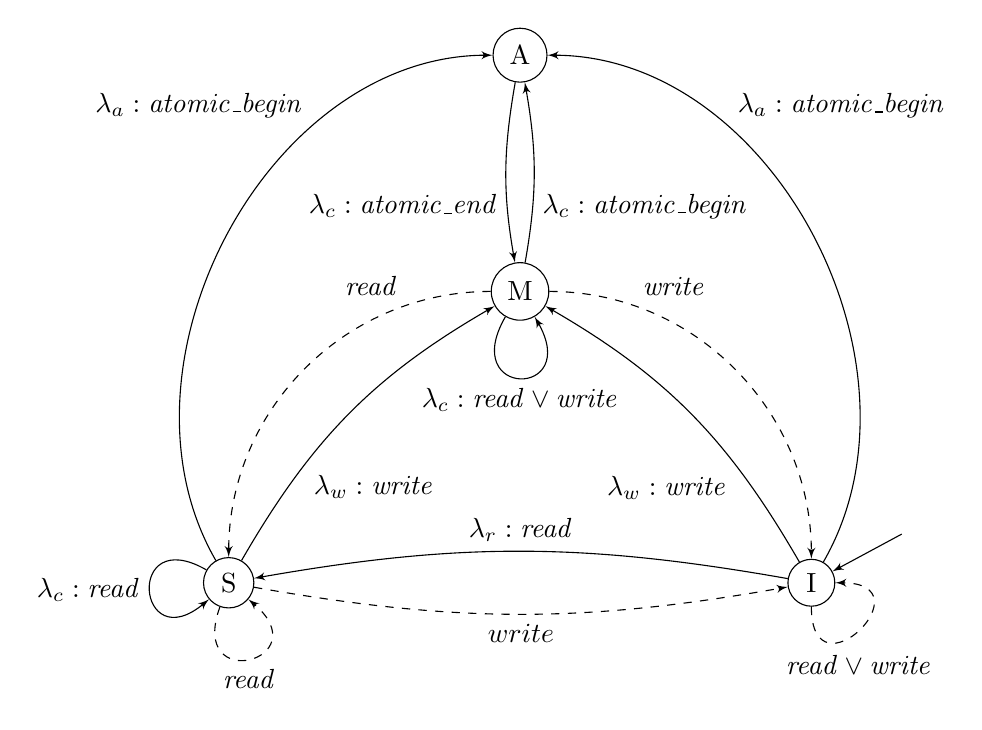
\begin{tikzpicture}[]

% nodes
\node [o]            at (  0  ,  3   ) (A)    {A};
\node [o]            at (  0  ,  0   ) (M)    {M};
\node [o]            at ( -3.7, -3.7 ) (S)    {S};
\node [o]            at (  3.7, -3.7 ) (I)    {I};
\node [o, draw=none] at (  5.0, -3.0 ) (init) {};

%  edges
\path [->]
  (init) edge                                                 node []                     {}                                     (I)

  (A)    edge [in=100, out=260]                               node [left       , pos=0.7] {$\lambda_c : \mathit{atomic\_end}$}   (M)

  (M)    edge [in=-80, out=80]                                node [right      , pos=0.3] {$\lambda_c: \mathit{atomic\_begin}$}  (A)
  (M)    edge [loop, distance=1.2cm, in=-60, out=240]         node [below] {$\lambda_c: \mathit{read} \lor \mathit{write}$}      (M)
  (M)    edge [dashed, in=90, out=180]                        node [above left , pos=0.2] {$\mathit{read}$}                      (S)
  (M)    edge [dashed, in=90, out=0]                          node [above right, pos=0.2] {$\mathit{write}$}                     (I)

  (S)    edge [in=180, out=120]                               node [above left , pos=0.7] {$\lambda_a : \mathit{atomic\_begin}$} (A)
  (S)    edge [in=210, out=60]                                node [below right, pos=0.3] {$\lambda_w : \mathit{write}$}         (M)
  (S)    edge [loop, distance=1.2cm, in=220, out=150]         node [left]                 {$\lambda_c : \mathit{read}$}          (S)
  (S)    edge [loop, dashed, distance=1.2cm, in=320, out=250] node [below]                {$\mathit{read}$}                      (S)
  (S)    edge [dashed, in=190, out=-10]                       node [below]                {$write$}                              (I)

  (I)    edge [in=0, out=60]                                  node [above right,pos=0.7]  {$\lambda_a : \mathit{atomic\_begin}$} (A)
  (I)    edge [in=-30, out=120]                               node [below left ,pos=0.3]  {$\lambda_w : \mathit{write}$}         (M)
  (I)    edge [in=10, out=170]                                node [above]                {$\lambda_r : \mathit{read}$}          (S)
  (I)    edge [loop, dashed, distance=1.2cm, in=0, out=-90]   node [below=0.2cm]          {$\mathit{read} \lor \mathit{write}$}  (I);

\end{tikzpicture}

			\caption{CTMC module of a shared memory variable}
			\label{fig:model-shared-memory}
		\end{figure}
	\item For example if a core reads a variable, it first needs to make sure that all other cores take notice and change its cache line copy state to shared in case it was modified before. After this the core fetches the cache line, marks its copy shared and continues reading the variable.
	\item taken from complex-lab, rephrase: The timings of shared read and shared write are as follows. A read on a modified or shared variable does not imply any extra work. It can immediately use the cached data. Therefore we consider this operation instantaneous. If a read is done on an invalid copy, it has to first fetch an up-to-date copy of the cache line and make sure all other cores are notified before it can proceed. This usually takes around 50 CPU cycles. A write on a modified variable is instantaneous, since all other cores do not have an up-to-date copy and therefore do not have to be notified. If the cache line in question is in a shared or invalid state, we first have to wait until all other cores follow the request to invalidate their copies of the cache line. After this we can safely mark our copy modified and write to it. This operation usually takes around 100 cycles.
	\item taken from complex-lab, rephrase: The number of cycles these operations take is strongly dependent on the CPU itself. For the CTMC model we assume a cache read to use 50 cycles and a cache write to use 100 cycles. The rates of the transitions corresponding to the described events is then the reciprocal of the cycle time: 1, $\frac{1}{50}$ or $\frac{1}{100}$.
	\item $\lambda_c$, $\lambda_r$, $\lambda_w$, $\lambda_a$ one cycle, read, write, atomic\_begin rate. Reciprocal of the average number of cycles needed for each of these actions
	\item explain CTMC behaviour and work around through setting atomic\_begin to something higher than write, although normally it would be just that
	\item explain to move atomic rate to atomic end to make parallel and serial code look different (explain how parallel and serial doesn't make a difference for interleaved CTMCs)
\end{itemize}

%%%%%%%%%%
\paragraph{Central Counter Barrier}
\label{sssec:analysis-modelchecking-modelling-central-counter}
\begin{itemize}
	\item repeat variables and initial configuration from the algorithm box
	\item Algorithm explained in Section~\ref{sssec:background-currently-used-shared}
	\item Control flow diagram Figure~\ref{fig:model-central-counter}
		\begin{figure}[htbp]
			\centering
			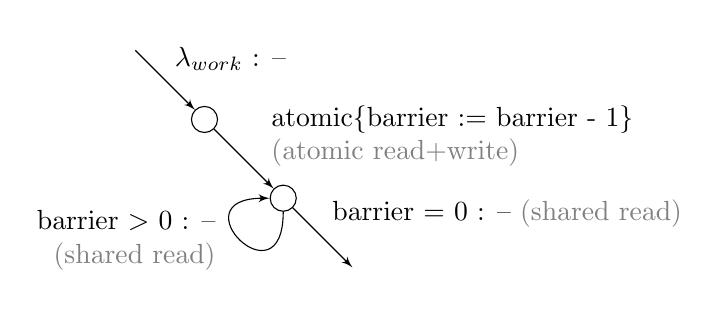
\begin{tikzpicture}[node distance = 2.0cm, auto]

% nodes
\node [o, draw=none] at ( 0 ,  0 ) (init) {};
\node [o]            at ( 1 , -1 ) (1)    {};
\node [o]            at ( 2 , -2 ) (2)    {};
\node [o, draw=none] at ( 3 , -3 ) (done) {};

%  edges
\path [->] (init) edge   node                       {$\lambda_{work}$ : --}                        (1)
           (1)    edge   node [pos=0.8, align=left] {atomic\{barrier := barrier - 1\} \\ \color{gray} (atomic read+write)} (2)
           (2)    edge [loop, distance=1.2cm, out=-90, in=180] node [left=0.2cm, align=right] {barrier $>$ 0 : -- \\ \color{gray}(shared read)} (2)
           (2)    edge   node                       {barrier = 0 : -- \color{gray}(shared read)}   (done);

\end{tikzpicture}

			\caption{Control flow diagram of the Central Counter Barrier}
			\label{fig:model-central-counter}
		\end{figure}
	\item rates for reading writing and atomic operations are determined by the module for the shared variable \texttt{barrier}
	\item the synchronization to the shared variable module is hinted at in grey
	\item The control flow has been augmented by one rate that the resulting CTMC will use. $\lambda_{work}$ is the work rate, meaning the time spent doing actual work. It is used to add an initial distribution to the model so that we can control how the arrival times of the threads at the barrier are distributed. In particular not all threads arrive at the exact same instant in time at the barrier, which is an extreme case.
	\item atomic op consists of multiple smaller transitions: begin atomic (locks the variable), read, decrement, write, end atomic (releases the lock).
	\item functional model does resetting and repetition. Three barriers, as described in~\ref{ssec:building-blocks}. (if you did not describe it there, you have to do it here)
\end{itemize}

%%%%%%%%%%
\paragraph{Ronny's simple barrier}
\label{ssssec:analysis-modelchecking-modelling-ronny-simple}
\begin{itemize}
	\item repeat variables and initial configuration from the algorithm box
	\item Algorithm explained in Section~\ref{ssec:new-simple}
	\item Control flow diagram Figure~\ref{fig:model-ronny-simple}
		\begin{figure}[htbp]
			\centering
			%
% does not 100% reflect the prism model
%

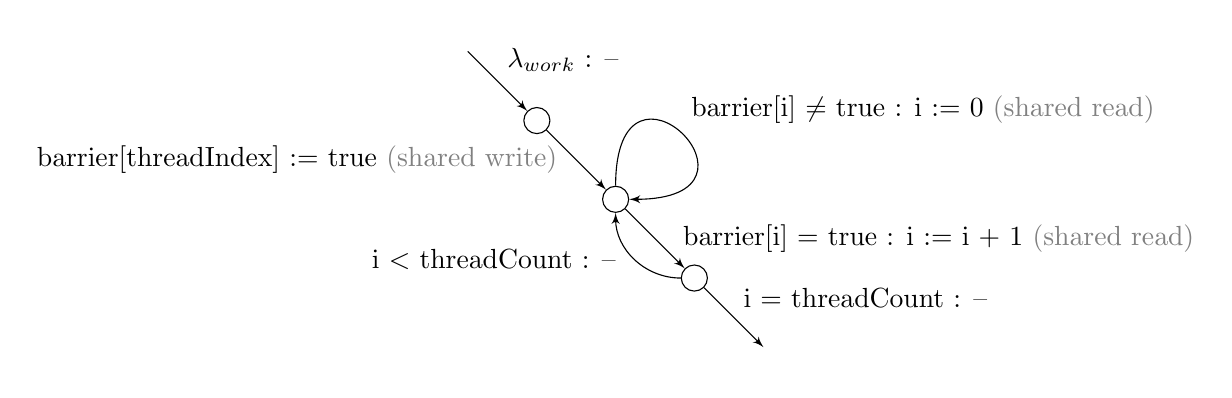
\begin{tikzpicture}[node distance = 2.0cm, auto]

% nodes
\node [o, draw=none] at ( 0   ,  0  ) (init) {};
\node [o]            at ( 1   , -1  ) (1)    {};
\node [o]            at ( 2   , -2  ) (2)    {};
\node [o]            at ( 3   , -3  ) (3)    {};
\node [o, draw=none] at ( 4   , -4  ) (done) {};

%  edges
\path [->] (init) edge                                      node        {$\lambda_{work}$ : --}                                      (1)
           (1)    edge                                      node[left]  {barrier[threadIndex] := true \color{gray}(shared write)~~}  (2)
           (2)    edge [loop, distance=2cm, out=90, in=0] node          {barrier[i] $\ne$ true : i := 0 \color{gray}(shared read)}   (2)
           (2)    edge                                      node[right] {~~barrier[i] = true : i := i + 1 \color{gray}(shared read)} (3)
           (3)    edge [out=180, in=-90]                    node[left]  {i $<$ threadCount : --~~}                                   (2)
           (3)    edge                                      node        {i = threadCount : --}                                       (done);

\end{tikzpicture}

			\caption{Control flow diagram of Ronny's simple barrier}
			\label{fig:model-ronny-simple}
		\end{figure}
	\item each element of the array \texttt{barrier} is located in an own cache line. Therefore each thread has \texttt{threadCount} cache line copy modules, one for each element in the array. In total a CTMC model of this protocol has $\mathtt{threadCount}^2$ cache line copy modules plus $\mathtt{threadCount}$ thread modules.
	\item As described in the previous paragraph, $\lambda_{work}$ is the work rate and all other rates are determined by the cache line copy modules.
	\item functional model does resetting and repetition using a counter instead of bools as described in Section~\ref{ssec:building-blocks} (if you did not describe it there, you have to do it here)
	\item functional model splits some of the transitions to allow for more interleaving, thus more errors can be revealed.
\end{itemize}

%%%%%%%%%%
\paragraph{Dissemination Barrier}
\label{ssssec:analysis-modelchecking-modelling-dissemination}
\begin{itemize}
	\item repeat variables and initial configuration from the algorithm box
	\item no special module for distributed memory, since all variables are independently stored in the local memory of each process. There is no influence that copies data between processes other then the user-specified program itself.
	\item Algorithm explained in Section~\ref{sssec:background-currently-used-distributed}
	\item Control flow diagram augmented with rates: Figure~\ref{fig:model-dissemination}
		\begin{figure}[htbp]
			\centering
			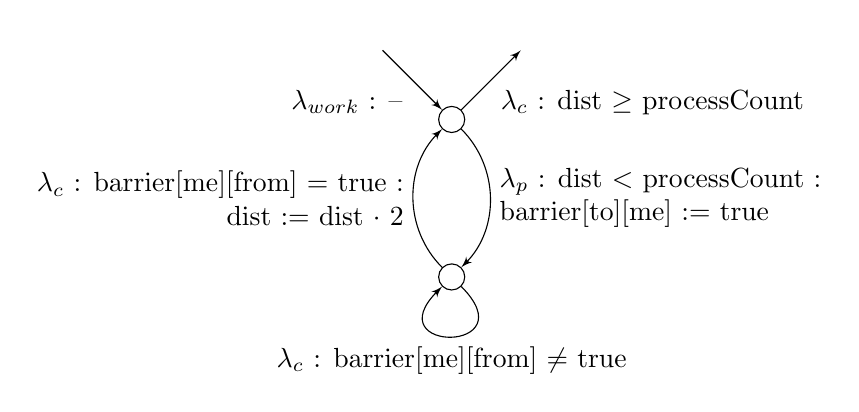
\begin{tikzpicture}[auto]

% nodes
\node [o, draw=none] at (  0 ,  0 ) (init) {};
\node [o]            at (  1 , -1 ) (1)    {};
\node [o]            at (  1 , -3 ) (2)    {};
\node [o, draw=none] at (  2 ,  0 ) (done) {};
%  edges
\path [->] (init) edge                  node [below left] {$\lambda_{work}$ : --} (1)

           (1)    edge node [below right] {$\lambda_c$ : dist $\ge$ processCount} (done)

           (1)    edge [out=-45, in=45] node [right, align=left] {$\lambda_p$ : dist $<$ processCount : \\ barrier[to][me] := true} (2)


           (2)    edge [loop, distance=1.2cm, out=315, in=225] node[below] {$\lambda_c$ : barrier[me][from] $\ne$ true} (2)

           (2)    edge [out=135, in=225] node[left, align=right]  {$\lambda_c$ : barrier[me][from] = true : \\ dist := dist $\cdot$ 2} (1);

\end{tikzpicture}

			\caption{Augmented Control flow diagram of the Dissemination Barrier}
			\label{fig:model-dissemination}
		\end{figure}
	\item As in the two previous paragraphs $\lambda_{work}$ is the work rate.
	\item we assume all local operations to be much quicker, ten to a thousand times, than remote operations. Therefore we assign the rate $\lambda_c$ (one CPU cycle) to local operations. $\lambda_p$, which is assigned to remote write (put) operations, is assigned a rate of $\frac{1}{100}$. This value is, like the shared memory rates, hardware-dependent. For simplicity's sake we therefore assume a remote transfer to take 100 cycles.
	\item one could make this more fine grained by introducing separate rates for local reading and writing.
	\item \texttt{to} and \texttt{from} are shorthands for \texttt{processIndex $\pm$ dist (mod processCount)}
	\item In the CTMC model, resulting from unwinding this control flow diagram, a put onto a remote process is represented as a synchronized action, so the target process stores the new value in its CTMC module.
	\item functional model does resetting and repetition with a counter instead of bools as described in Section~\ref{ssec:building-blocks}.
\end{itemize}

%%%%%%%%%%
\paragraph{Ronny fancy barrier}
\label{ssssec:analysis-modelchecking-modelling-ronny-fancy}
\begin{itemize}
	\item repeat variables and initial configuration from the algorithm box
	\item Algorithm explained in Section~\ref{ssec:new-fancy}
	\item Control flow diagram augmented with rates: Figure~\ref{fig:model-ronny-fancy}
		\begin{figure}[htbp]
			\centering
			%
% does not 100% reflect the prism model
%

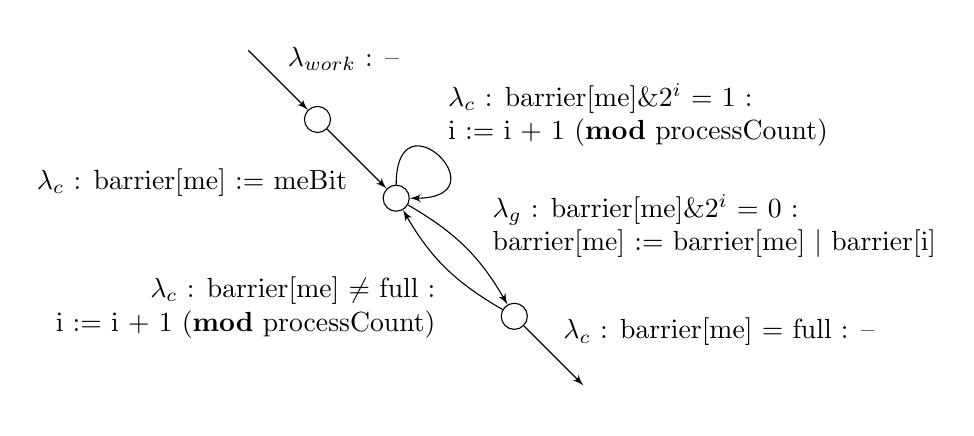
\begin{tikzpicture}[auto]

% nodes
\node [o, draw=none] at (   0 ,   0 )     (init) {};
\node [o]            at (   1.0 ,  -1.0 ) (1)    {};
\node [o]            at (   2.0 ,  -2.0 ) (2)    {};
\node [o]            at (   3.5 ,  -3.5 ) (3)    {};
\node [o, draw=none] at (   4.5 ,  -4.5 ) (done) {};

%  edges
\path [->]
  (init) edge                                      node [above right]             {$\lambda_{work}$ : --}                     (1)

  (1)    edge                                      node [below left]              {$\lambda_c$ : barrier[me] := meBit}        (2)

  (2)    edge [loop, distance=1.2cm, out=90, in=0] node [above right, align=left] {$\lambda_c$ : barrier[me]\&2$^i$ = 1 : \\ i := i + 1 (\textbf{mod} processCount)} (2)

  (2)    edge [out=-30, in=120] node [above right, pos=0.7, align=left] {$\lambda_g$ : barrier[me]\&2$^i$ = 0 : \\ barrier[me] := barrier[me] \textbar~barrier[i] } (3)

  (3)    edge [out=150, in=300]                    node [below left, align=right]  {$\lambda_c$ : barrier[me] $\ne$ full : \\ i := i + 1 (\textbf{mod} processCount)} (2)

  (3)    edge []                                   node [above right, align=left] {$\lambda_c$ : barrier[me] = full : --}     (done);


\end{tikzpicture}

			\caption{Augmented Control flow diagram of Ronny's fancy barrier}
			\label{fig:model-ronny-fancy}
		\end{figure}
	\item Rates are like in previous section, except we now use remote read (get) with a rate of $\lambda_g = \frac{1}{100}$.
	\item functional model does resetting and repetition using three barriers as described in~\ref{ssec:building-blocks}.
\end{itemize}

%%%%%%%%%%%%%%%%%%%%
\subsubsection{Functional properties}
\label{sssec:analysis-modelchecking-functional-properties}
\begin{itemize}
	\item intro text here
	\item in this section we will use \emph{thread} and \emph{process} interchangeable, because for the modelling side the wording makes no difference.
	\item LTL as logic, Spin as model checker
	\item $T$ is the set of all threads
	\item $\mathit{left_t}$ is a predicate describing all states where thread $t$ has passed the barrier
	\item $entered_t$ is a predicate describing all states where thread $t$ has passed the initial work period and therefore entered the barrier.
	\item \textbf{A:} \emph{a thread may only exit the barrier if all threads have entered it}
		\begin{center}
			$\square \big( ~ ( \exists t \in T . \mathit{left_t} ) \implies \forall s \in T. \mathit{entered_s} ~ \big)$
		\end{center}
	\item \textbf{B:} \emph{if all threads entered the barrier, they will all leave it in a finite amount of time}
		\begin{center}
			$\square \big( ~(\forall t \in T . \mathit{entered_t} ) \implies \forall s \in T. \lozenge \mathit{left_s} ~ \big)$
		\end{center}
	\item A and B are the two basic properties a barrier protocol must satisfy
	\item A could be seen as safety and B as liveness of a barrier protocol
	\item yes it works.
\end{itemize}

%%%%%%%%%%%%%%%%%%%%
\subsubsection{Quantitative properties}
\label{sssec:analysis-modelchecking-quantitative-properties}
\begin{itemize}
	\item intro text here
	\item in this section we will use \emph{thread} and \emph{process} interchangeably, because for the modelling side the wording makes no difference. (same is in section before)
	\item CSRL as logic, PRISM as model checker
\end{itemize}

%%%%%%%%%%
\paragraph{Identification and formalisation}
\label{ssssec:analysis-modelchecking-quantitative-properties-identification}
\begin{itemize}
	\item interesting values to query for
		\begin{itemize}
			\item time: unit: CPU cycles. srew 1.
			\item energy consumption: unit: Joule, and rate of energy consumption: unit: Joule per second = Watt. (assume 2.5ghz. W (nJ/ns) = 2.5 * nJ/cycle)
				\begin{itemize}
					\item trew shared memory operations = 200nJ
					\item trew cached shared memory operation = 2nJ
					\item trew any other operation = 0nJ
					\item for dist: remote 200nJ, local memory op = 2nJ, others none
					\item baseline of 11W
					\item These numbers are a very limited estimate derived from a small reference measurement. The numbers can be found in Section~\ref{ssec:energy-measurement}.
				\end{itemize}
			\item (diss, ronny's fancy) number of remote transfers. trew for remote operations = 1. srew =0.
		\end{itemize}
	\item interesting points in time
		\begin{itemize}
			\item (A) first thread entered the barrier
			\item (B) last thread entered the barrier
			\item (C) first thread left the barrier
			\item (D) last thread left the barrier
			\item (W) (only for Central Counter and ronny's simple) the last thread finished writing
			\item (R$i$) (only for Dissemination) last process left round $i$, i.e. entered round $i+1$. The current round of process is determined through the variable $\mathit{dist}$. $\mathit{round} = 1 + \log_2 \mathit{dist}$.
		\end{itemize}
	\item resulting properties
		\begin{itemize}
			\item $T$ is the set of all threads
			\item \textbf{A:} \emph{Average reward until the first thread enters the barrier}
				\begin{center}
					$\mathrm{ReaRew}(\exists t \in T . \mathit{entered_t} )$
				\end{center}
			\item \textbf{B:} \emph{Average reward until the last thread enters the barrier}
				\begin{center}
					$\mathrm{ReaRew}(\forall t \in T . \mathit{entered_t} )$
				\end{center}
			\item \textbf{C:} \emph{Average reward until the first thread leaves the barrier}
				\begin{center}
					$\mathrm{ReaRew}(\exists t \in T . \mathit{left_t} )$
				\end{center}
			\item \textbf{D:} \emph{Average reward until the last thread leaves the barrier}
				\begin{center}
					$\mathrm{ReaRew}(\forall t \in T . \mathit{left_t} )$
				\end{center}
			\item \textbf{W:} \emph{Average reward until the last thread finished writing}
				\begin{center}
					$\mathrm{ReaRew}(\forall t \in T . \mathit{done\_writing_t} )$
				\end{center}
			\item \textbf{R$i$:} \emph{Average reward until the last thread left round $i$}
				\begin{center}
					$\mathrm{ReaRew}(\forall t \in T . \mathit{left\_round_{i,t}} )$
				\end{center}
			\item where the predicates have the obvious meaning.
			\item and combinations of these to get measures like (D-B) last in until last out.
		\end{itemize}
	\item which parameters to variate
		\begin{itemize}
			\item thread count. Maximum 4 is almost always considered. Model checking limitations bla.
			\item work rate. Variate the distribution of the times the threads enter the barrier.
		\end{itemize}
\end{itemize}

%%%%%%%%%%
\paragraph{Evaluation}
\label{ssssec:analysis-modelchecking-quantitative-properties-results}
\begin{itemize}
	\item 
\end{itemize}

%%%%%
\subparagraph{Shared memory barriers}
\label{sssssec:analysis-modelchecking-quantitative-properties-results-shared}
\begin{itemize}
	\item work = 100. Expected time it takes a thread to arrive at the barrier is 100 cycles.
	\item last to last, last to first Figure~\ref{fig:cs-time-work-100-B-C-D}
		\begin{figure}[htbp]
			\centering
			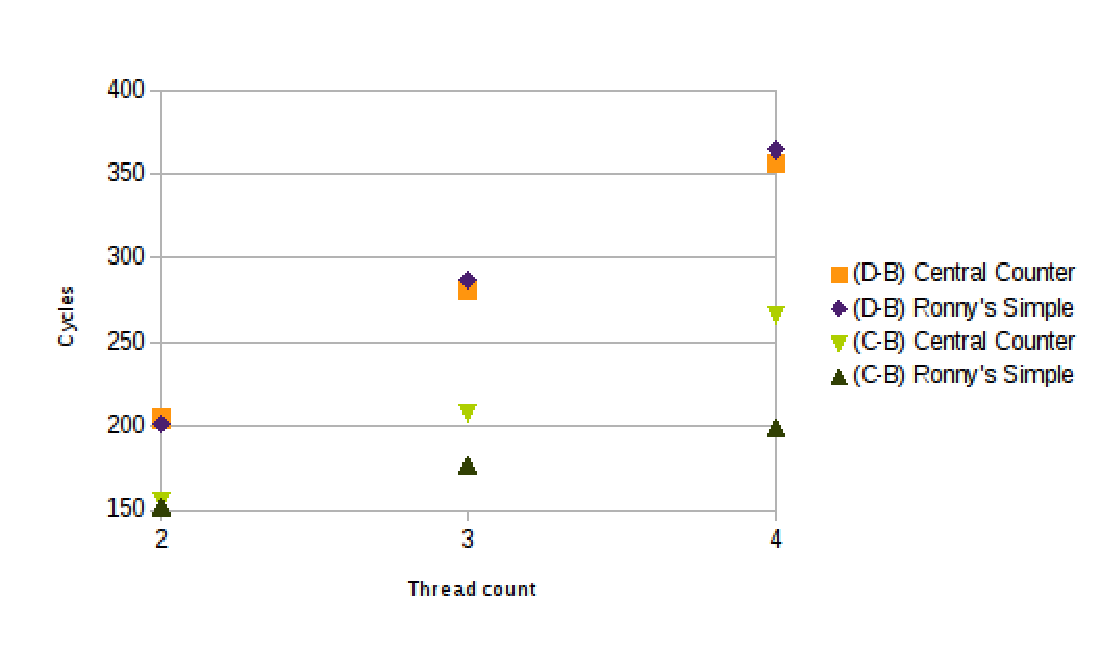
\includegraphics[width=10cm]{charts/cs-time-work-100-B-C-D}
			\caption{Expected execution time}
			\label{fig:cs-time-work-100-B-C-D}
		\end{figure}
		\begin{itemize}
			\item both barriers similarly fast when considering the last one to finish
			\item ronny's simple faster for the first one to leave
		\end{itemize}
	\item distribution of total time and energy spent: Figure~\ref{fig:cs-work-100-partition}
		\begin{figure}[htbp]
			\centering
			\begin{minipage}{0.53\linewidth}
				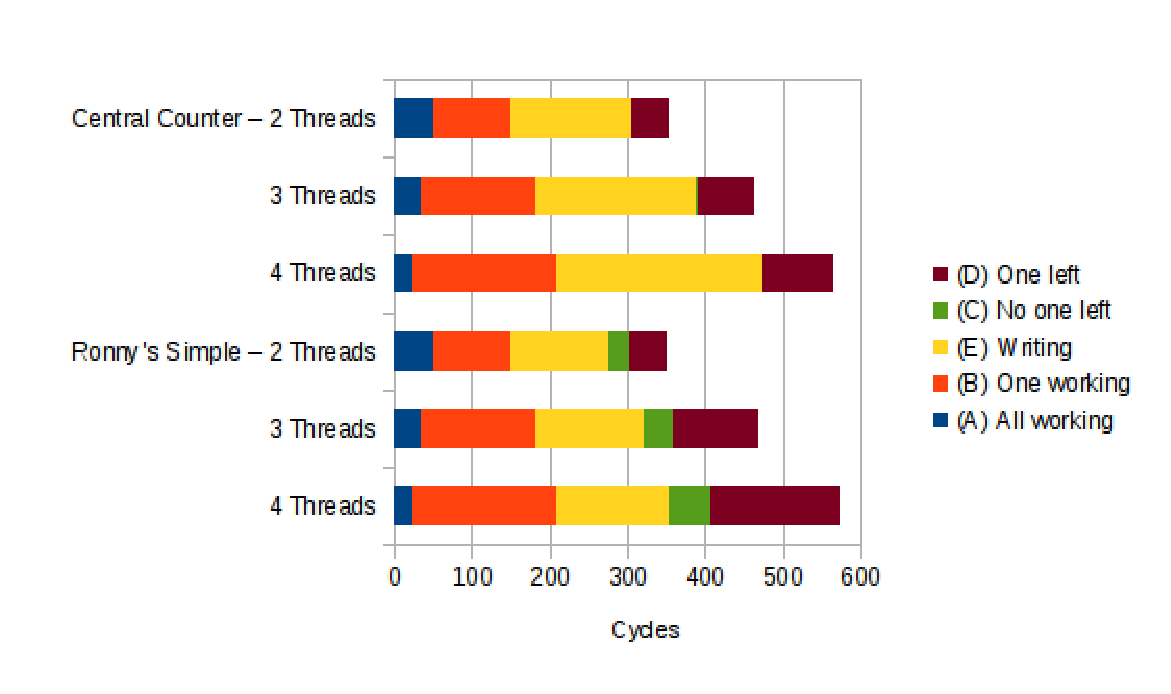
\includegraphics[height=4.3cm]{charts/cs-time-work-100-partition}
			\end{minipage}
			\begin{minipage}{0.46\linewidth}
				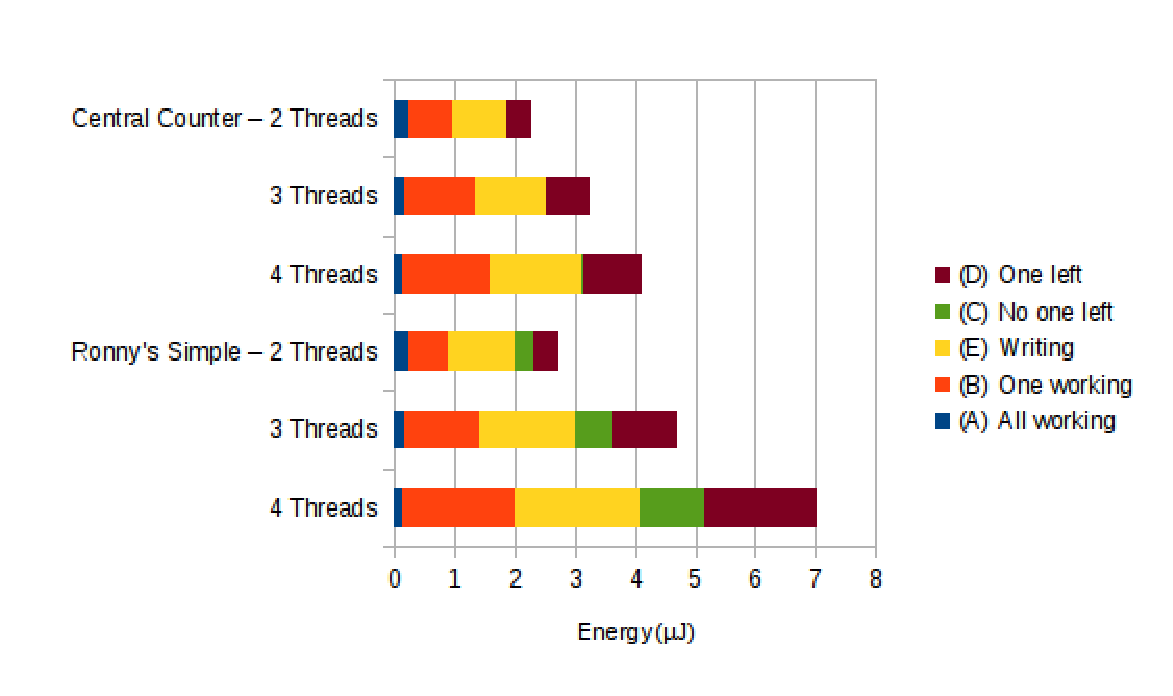
\includegraphics[height=4.3cm]{charts/cs-energy-work-100-partition}
			\end{minipage}
			\caption{Distribution of total time spent and energy consumed}
			\label{fig:cs-work-100-partition}
		\end{figure}
	\item time
		\begin{itemize}
			\item stacked fashion. Including the time of the previous bar.
			\item the initial work distribution is the same for all processes and protocols
			\item cc: first thread leaves a few cycles after writing is done. Because the last one to write its value will likely immediately read the completed barrier and leave.
			\item from the moment the first thread leaves, all threads only read. No one writes anymore.
			\item writing, as expected, takes longer for Central Counter and reading takes longer for ronny's simple
			\item all parts take longer with increasing thread count, since CTMC semantic (described in Section~\ref{sssec:analysis-modelchecking-preliminaries}) makes a transition get an exit rate of the sum of the rates of all enabled transitions.
			\item in particular, assume you have $n$ interleaved modules (or concurrent threads of execution) where one transition in each module is enabled. The exit rate of the first transition to be triggered is then  $n \cdot \lambda$. The expected time of a parallel execution of all transitions is $\sum_{i=1}^{n} \frac{1}{i \cdot \lambda}$ time rather than $\frac{1}{\lambda}$.
			\item for example the expected number of cycles for the first process to enter is $\approx \frac{100}{n}$. The last one is finished working after $\approx$ 150, 183 and 208 cycles, for two, three and four processes.
			\item Especially reading for Central Counter (2: 50, 3:75, 4:92 cycles). Normally this period is expected to be nearly the same for all thread counts.
			\item writing for ronny's simple is expected to take less time than shown here (100 across the board instead of 2:125, 3:138, 4:146), for the same reason as reading takes longer as expected for the Central Counter Barrier.
		\end{itemize}
	\item energy
		\begin{itemize}
			\item similar to time
			\item ronny's simple needs more energy. Because it performs more shared memory operations and more local operations in the same amount of time, where the Central Counter Barrier spends considerable time waiting for atomic operations to finish.
			\item Central Counter's energy scales similarly to time.
			\item amount of energy for ronny's simple grows faster than time needed.
			\item ronny's simple spends considerable energy from the last commitment to first leaving the barrier.
		\end{itemize}
	\item rate of power consumption per protocol phase: Figure~\ref{fig:cs-power-work-100}
		\begin{figure}[htbp]
			\centering
			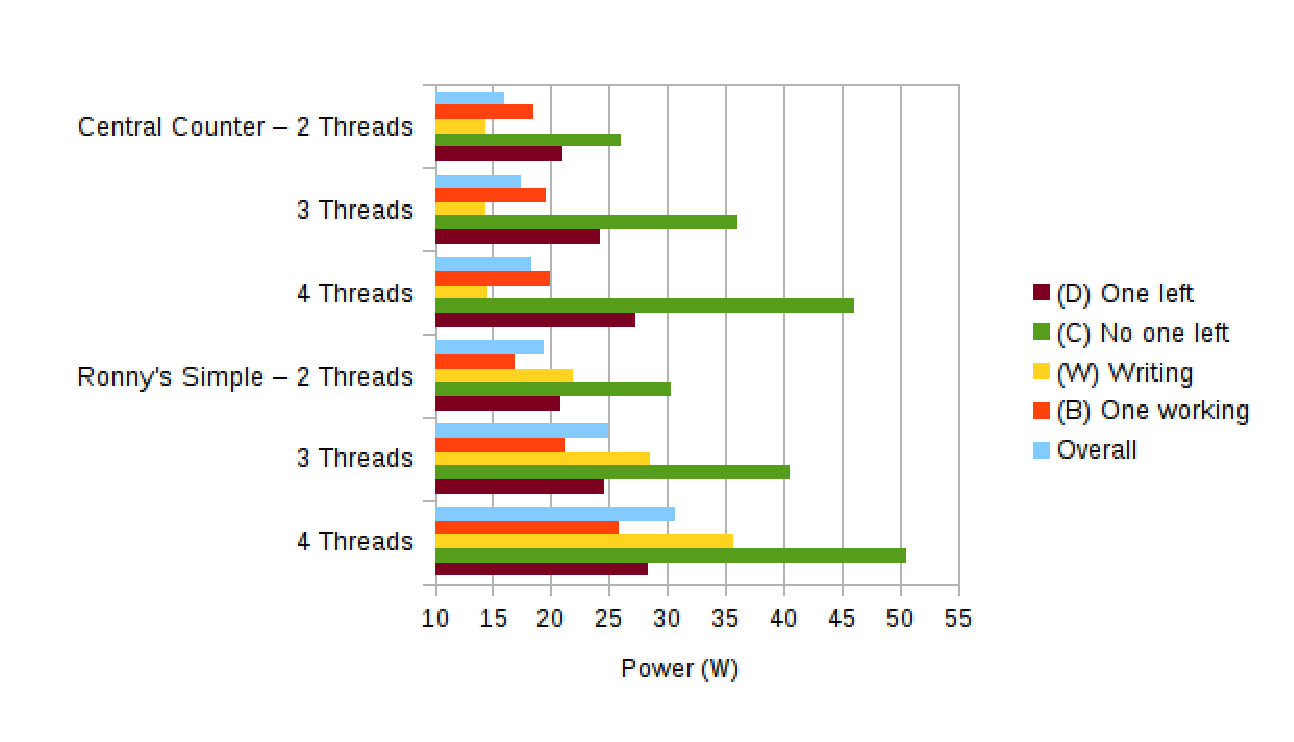
\includegraphics[width=10cm]{charts/cs-power-work-100}
			\caption{Rate of energy consumption for each phase}
			\label{fig:cs-power-work-100}
		\end{figure}
		\begin{itemize}
			\item same partitioning as the previous figure.
			\item (A) all working has 11W - the baseline.
			\item overall low for Central Counter (16-18.3W), ronny's simple (19.4 - 30.6)
			\item writing considerably higher for rs, because quicker and more shared memory operations.
			\item no one left: cc: high because very very short, rs: high because many shared reads across many threads.
			\item one left similar because cc: shared reads, rs: shared reads, and local reads.
		\end{itemize}
	\item reading vs writing: Figure~\ref{fig:cs-time-work-100-percent}
		\begin{figure}[htbp]
			\centering
			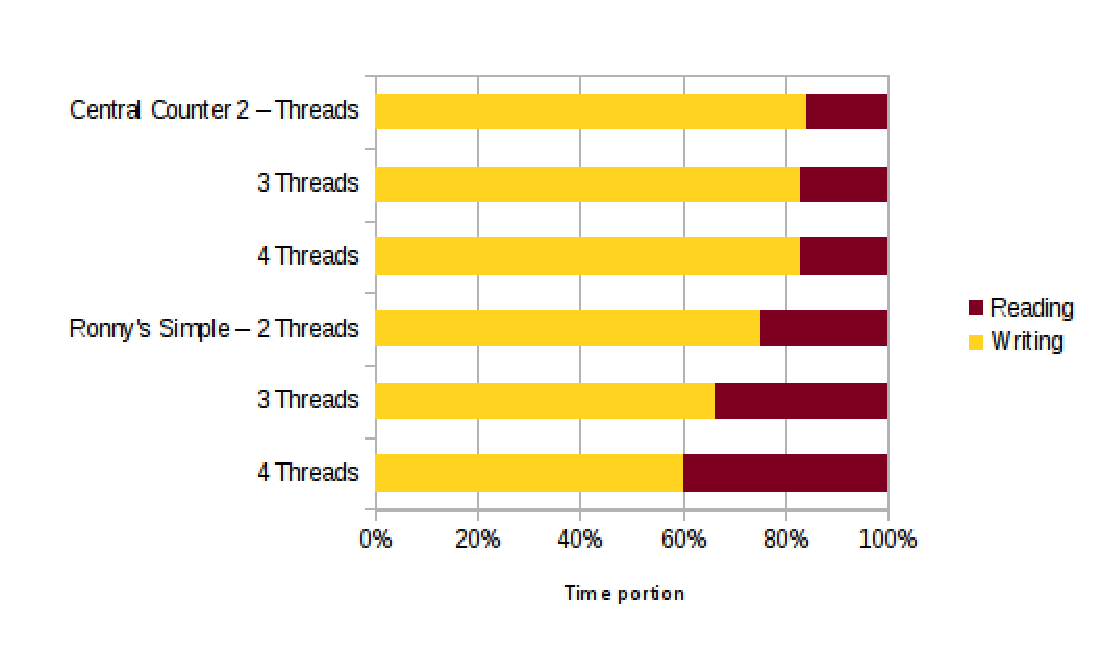
\includegraphics[width=10cm]{charts/cs-time-work-100-percent}
			\caption{Time spent reading versus writing}
			\label{fig:cs-time-work-100-percent}
		\end{figure}
		\begin{itemize}
			\item writing is from (A) to (W). Reading is from (W) to (D).
			\item with increasing thread count there is a shift from writing to reading in execution time.
		\end{itemize}
	\item work=1000. Still very small. (According to \cite{rab00} at a barrier each process spends on average 8194 CPU cycles idly\footnote{1813 microseconds accumulated idle time at 450MHz on 99.6 processes})
	\item last to last, last to first Figure~\ref{fig:cs-time-work-1000-B-C-D}
		\begin{figure}[htbp]
			\centering
			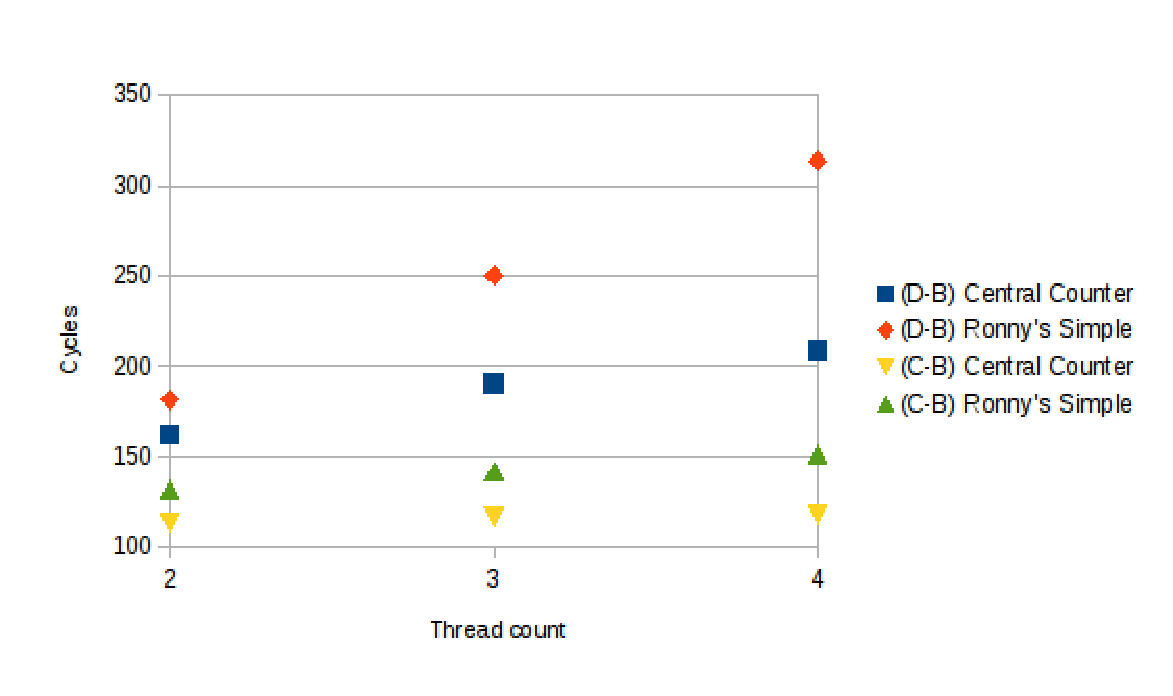
\includegraphics[width=10cm]{charts/cs-time-work-1000-B-C-D}
			\caption{Expected execution time}
			\label{fig:cs-time-work-1000-B-C-D}
		\end{figure}
		\begin{itemize}
			\item very different picture.
			\item Central Counter faster in all respects.
			\item probability of a thread trying to write while no one is writing at the moment increases due to the larger working period distribution. Writes for ronny simple tend to be serialized for the same reason, but ronny's simple still reads longer.
			\item time for one thread from entry to exit converges to one atomic op + a few cycles. 105 cycles for Central Counter.
		\end{itemize}
	\item distribution of total time and energy spent: Figure~\ref{fig:cs-work-1000-partition}
		\begin{figure}[htbp]
			\centering
			\begin{minipage}{0.53\linewidth}
				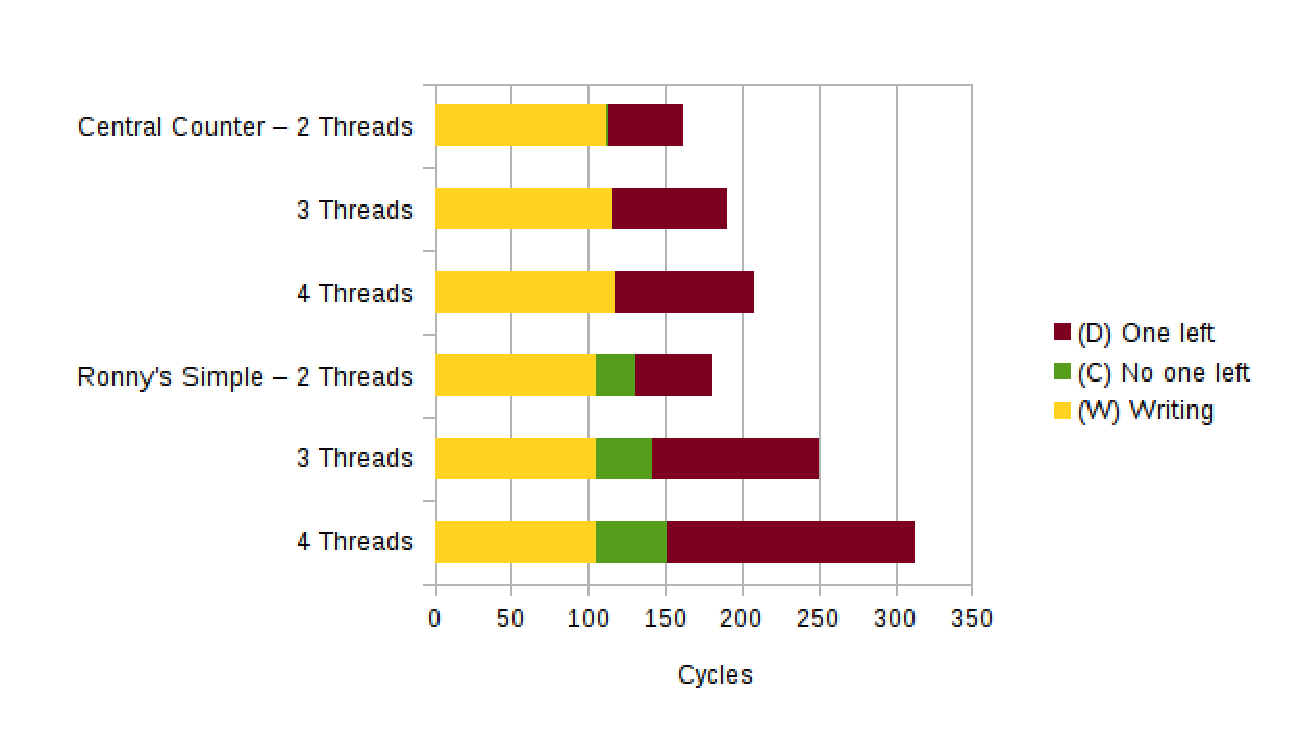
\includegraphics[height=4.3cm]{charts/cs-time-work-1000-partition}
			\end{minipage}
			\begin{minipage}{0.46\linewidth}
				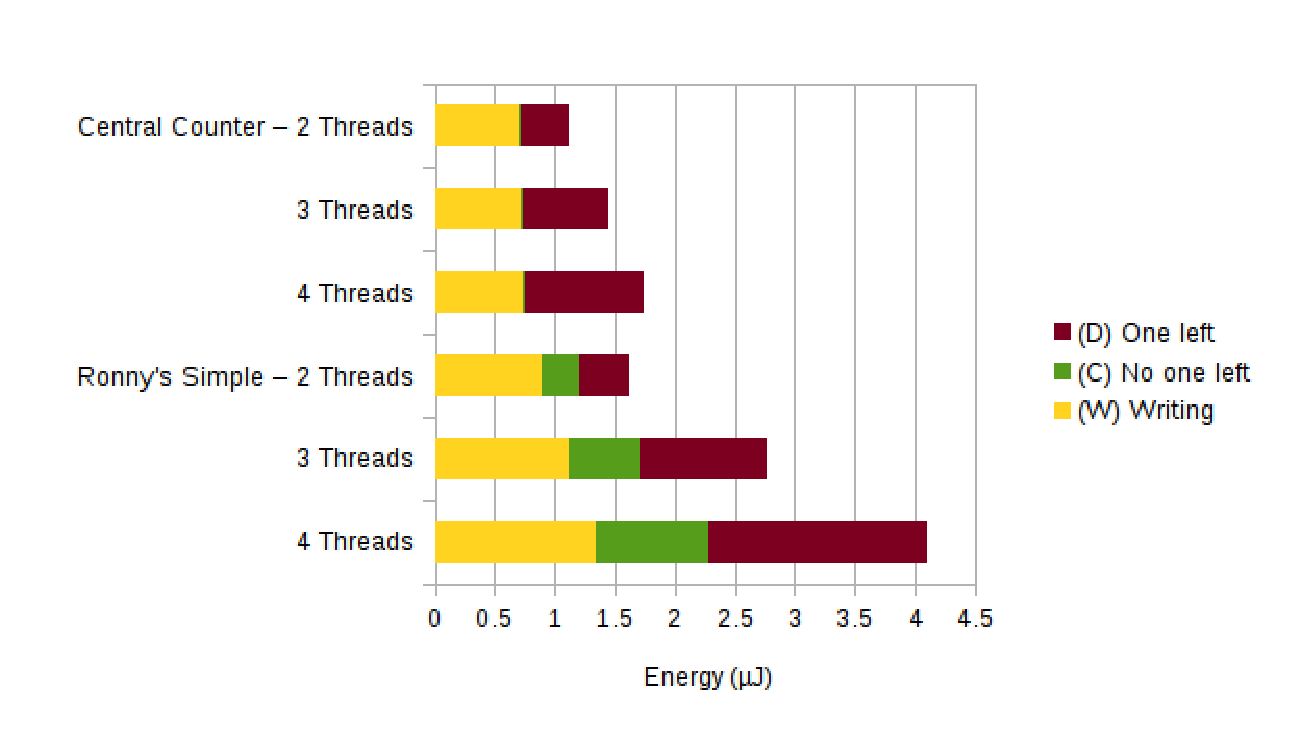
\includegraphics[height=4.3cm]{charts/cs-energy-work-1000-partition}
			\end{minipage}
			\caption{Distribution of total time spent and energy consumed}
			\label{fig:cs-work-1000-partition}
		\end{figure}
		\begin{itemize}
			\item Excluding (A) and (B) since they are large in comparison to the barrier
		\end{itemize}
	\item time
		\begin{itemize}
			\item as expected
		\end{itemize}
	\item energy
		\begin{itemize}
			\item writing is constant across multiple threads because the atomic op forbids reading the variable thus there is few busy waiting, whereas ronny's simple is constantly polling. And the amount increases with increasing thread count.
		\end{itemize}
	\item rate of power consumption per protocol phase: Figure~\ref{fig:cs-power-work-1000}
		\begin{figure}[htbp]
			\centering
			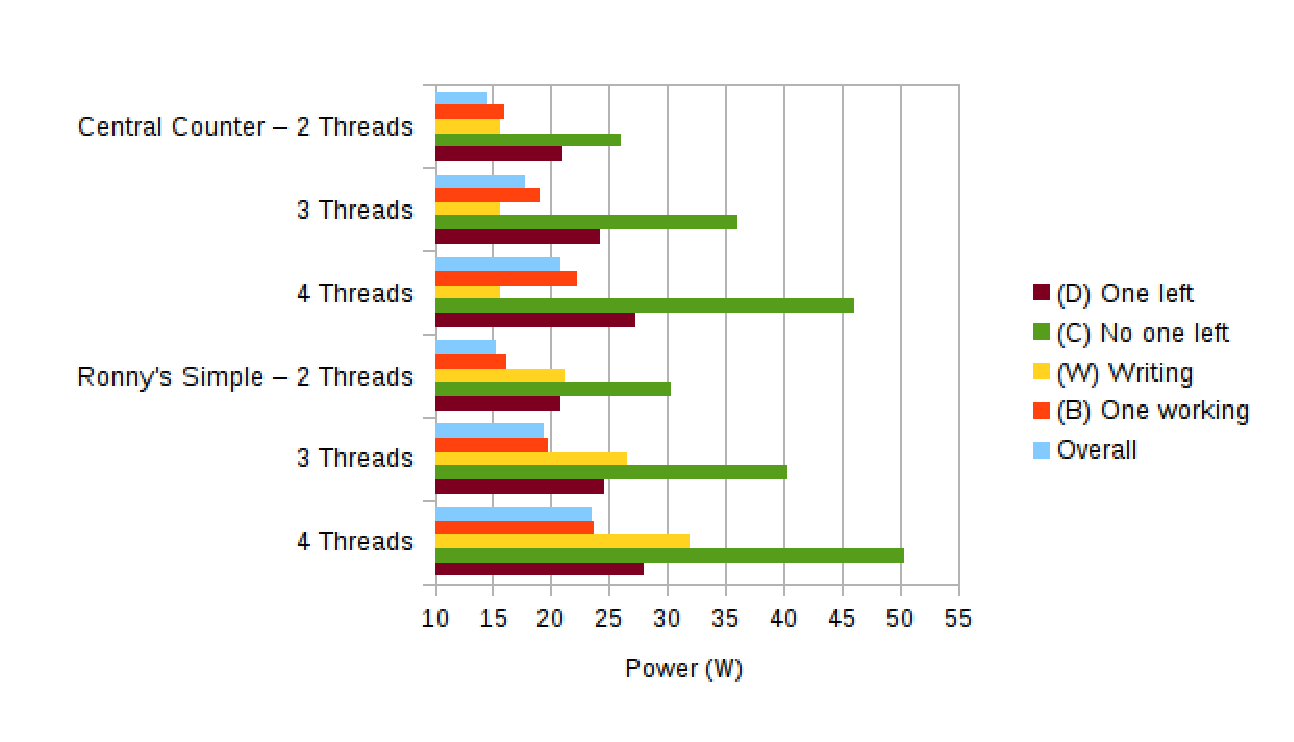
\includegraphics[width=10cm]{charts/cs-power-work-1000}
			\caption{Rate of energy consumption for each phase}
			\label{fig:cs-power-work-1000}
		\end{figure}
		\begin{itemize}
			\item more even. (1) longer work period. (2) cc and rs use similarly many shared and local operations (due to busy waiting) in the reading phase ((D) one left). Energy usage is dominated by busy waiting of threads.
			\item ronny's simple can catch up considerably. (cc:14.6-20.9, rs:15.3-23.5)
		\end{itemize}
	\item with larger and more realistic, since 1000 cycles is still very few, work periods this yields a series of writing operations for both algorithms, and a little more time spent reading for ronny's simple barrier.
\end{itemize}

%%%%%
\subparagraph{Distributed memory barriers}
\label{sssssec:analysis-modelchecking-quantitative-properties-results-distributed}
\begin{itemize}
	\item work = 100
	\item distribution of total time spent and total energy consumed: Figure~\ref{fig:df-work-100-partition}
		\begin{figure}[htbp]
			\centering
			\begin{minipage}{0.54\linewidth}
				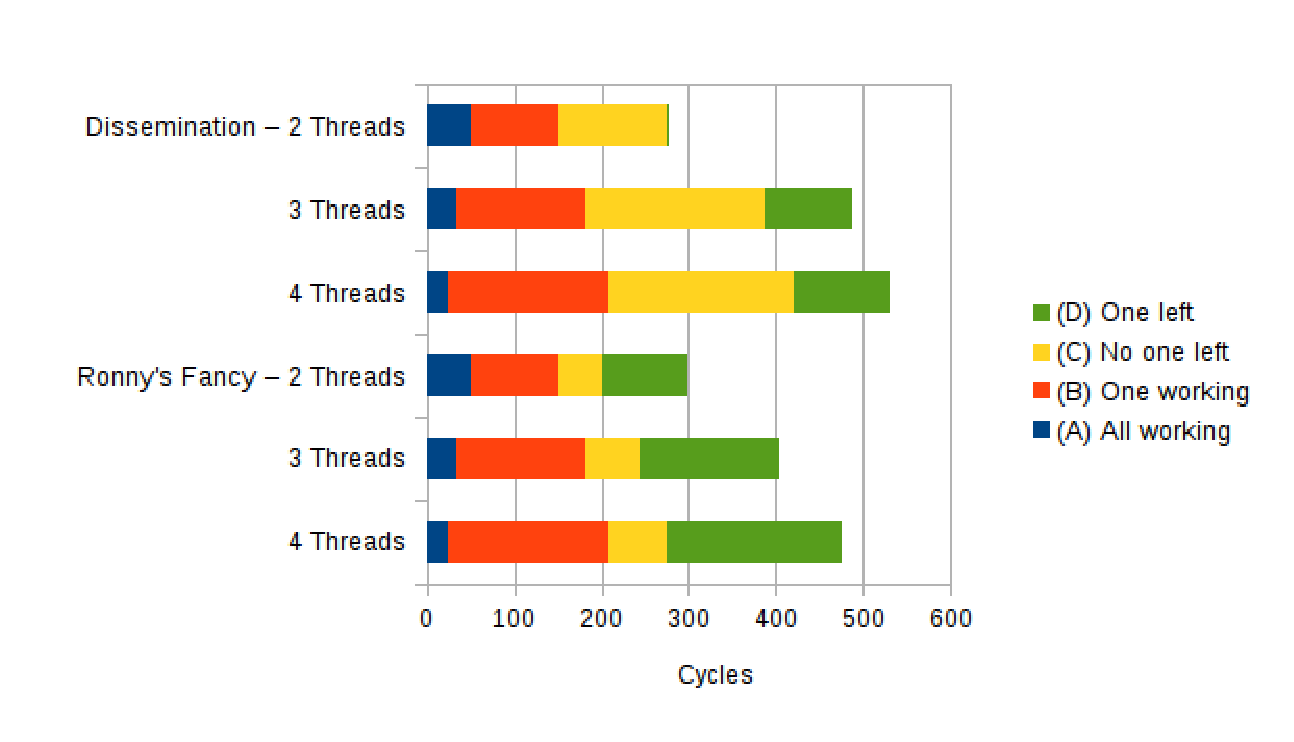
\includegraphics[height=4.3cm]{charts/df-time-work-100-partition}
			\end{minipage}
			\begin{minipage}{0.45\linewidth}
				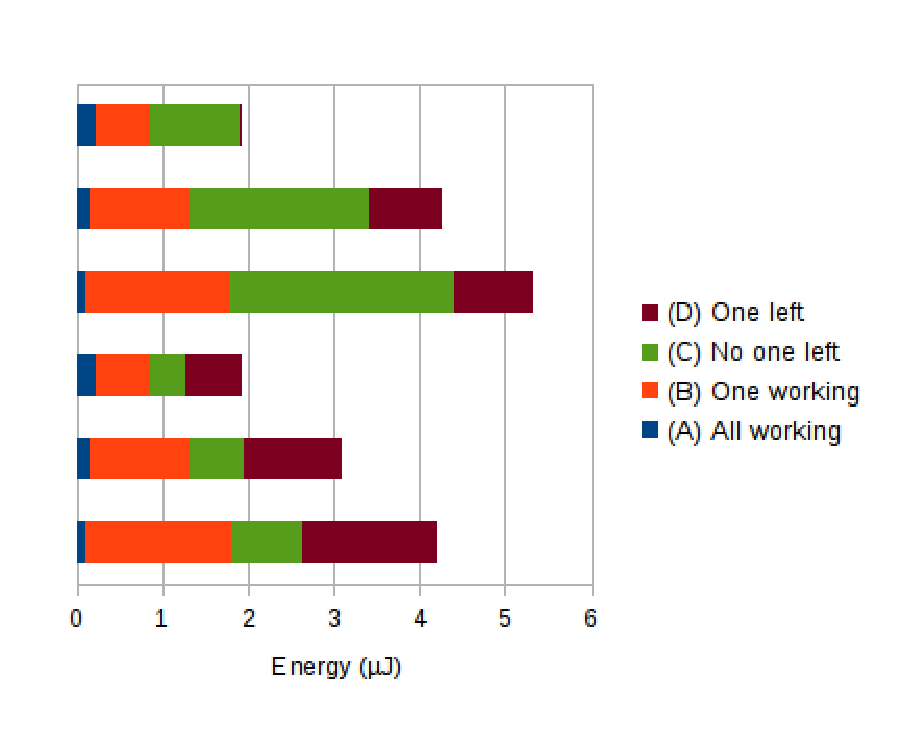
\includegraphics[height=4.3cm]{charts/df-energy-work-100-partition}
			\end{minipage}
			\caption{Distribution of total time spent and energy consumed}
			\label{fig:df-work-100-partition}
		\end{figure}
		\begin{itemize}
			\item ronny's fancy is quicker for process counts over two
			\item Dissemination finishes 23 cycles earlier than ronny's fancy for 2 processes because remote write can be executed during the work period of the other process, whereas ronny's simple still needs to execute 2 remote reads after the last process entered the barrier.
			\item rf: first one to leave unrealistic. Should not be quicker than 100 cycles. CTMC exit rate calculation.
			\item more time between first and last to leave.
			\item last and first exit at almost the same time for Dissemination, because when the second arrives and writes his part into the remote peers memory both will quickly exit. This cannot happen for processes since when the first leaves there might still be pending remote writes.
			\item energy consumption similar to time spent in proportion
		\end{itemize}
	\item Dissemination: distribution of total time spent and energy consumed: Figure~\ref{fig:d-work-100-partition}
		\begin{figure}[htbp]
			\centering
			\begin{minipage}{0.43\linewidth}
				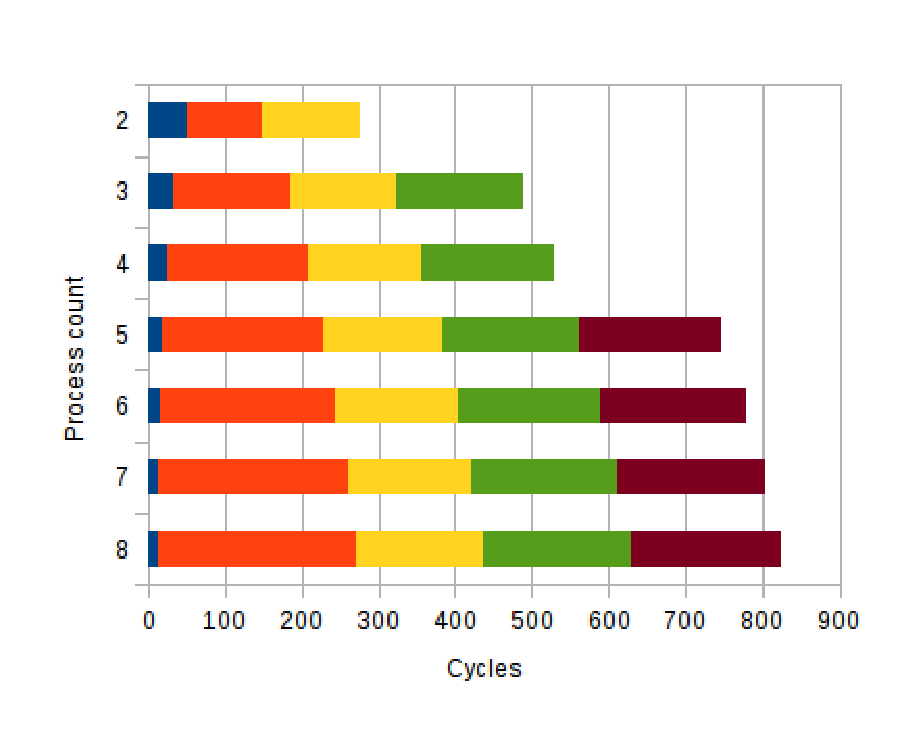
\includegraphics[height=4.2cm]{charts/d-time-work-100-partition}
			\end{minipage}
			\begin{minipage}{0.56\linewidth}
				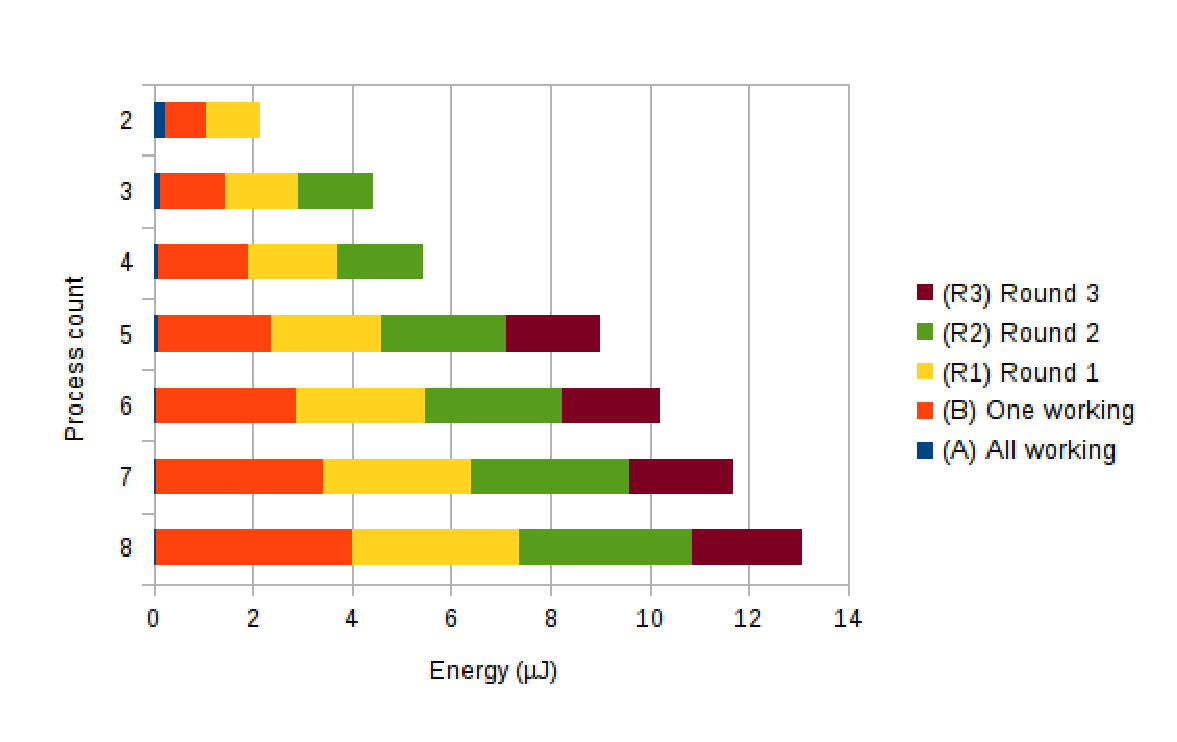
\includegraphics[height=4.2cm]{charts/d-energy-work-100-partition}
			\end{minipage}
			\caption{Distribution of total time spent and energy consumed for the Dissemination Barrier}
			\label{fig:d-work-100-partition}
		\end{figure}
		\begin{itemize}
			\item stair-esque running time due to $\lceil \log_2 \mathit{processCount} \rceil$ number of rounds. During those rounds remote writes are issued concurrently.
			\item unfavourable for non-power-of-two processes counts. Ref to Section~\ref{sssec:analysis-general-distributed}
			\item slight increase in per-round execution time with number of processes is result of CTMC interleaving semantics. This behaviour is realistic, because resource contention for remote writes and + non-uniform distribution durations for those writes, but we didn't specifically model this.
			\item energy consumption increase per round a bit larger than runtime increase. This is partly because more remote operations are issued as described in Section~\ref{ssssec:analysis-modelchecking-modelling-dissemination}. And partly because one more process is locally spinning before entering a new round.
		\end{itemize}
	\item rate of power consumption per phase: Figure~\ref{fig:df-power-work-100}
		\begin{figure}[htbp]
			\centering
			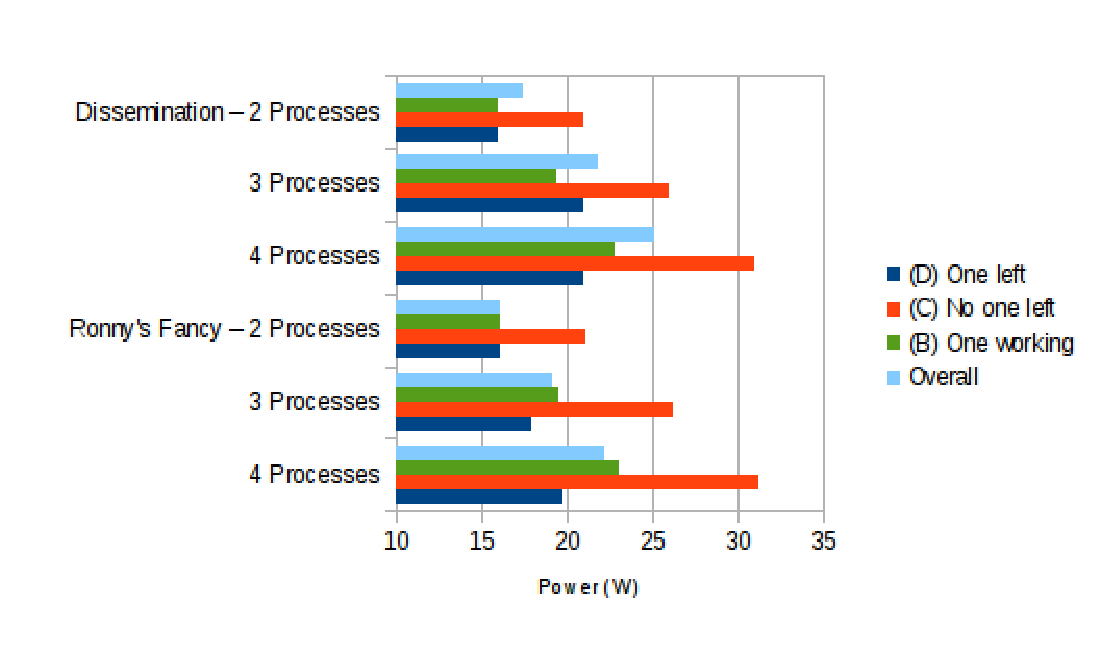
\includegraphics[width=10cm]{charts/df-power-work-100}
			\caption{Rate of energy consumption for each phase}
			\label{fig:df-power-work-100}
		\end{figure}
		\begin{itemize}
			\item All phases except the last are very similar.
			\item largely because comparing number of local and remote operations issued to the rewards given for these operations the amount of energy consumed is expected to be similar.
			\item Dissemination issues less remote operations, but due to local wait spinning a lot of local operations, ronny's fancy on the other hand polls remotely.
			\item in the last phase ronny's fancy draws less power because it takes a lot more time for a little more energy to be consumed.
			\item overall ronny's fancy performs slightly better.
		\end{itemize}
	\item longer work period. work=1000
	\item distribution of total time spent and energy consumed: Figure~\ref{fig:df-work-1000-partition}
		\begin{figure}[htbp]
			\centering
			\begin{minipage}{0.54\linewidth}
				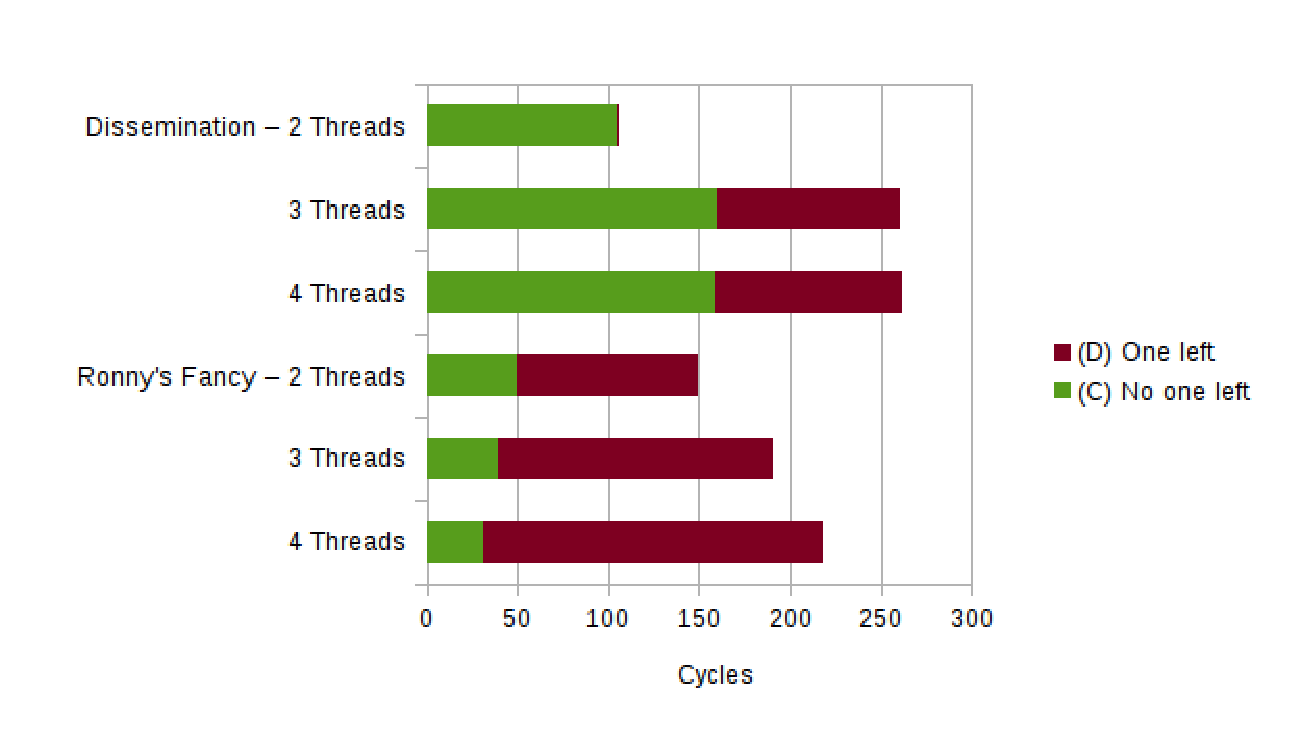
\includegraphics[height=4.3cm]{charts/df-time-work-1000-partition}
			\end{minipage}
			\begin{minipage}{0.45\linewidth}
				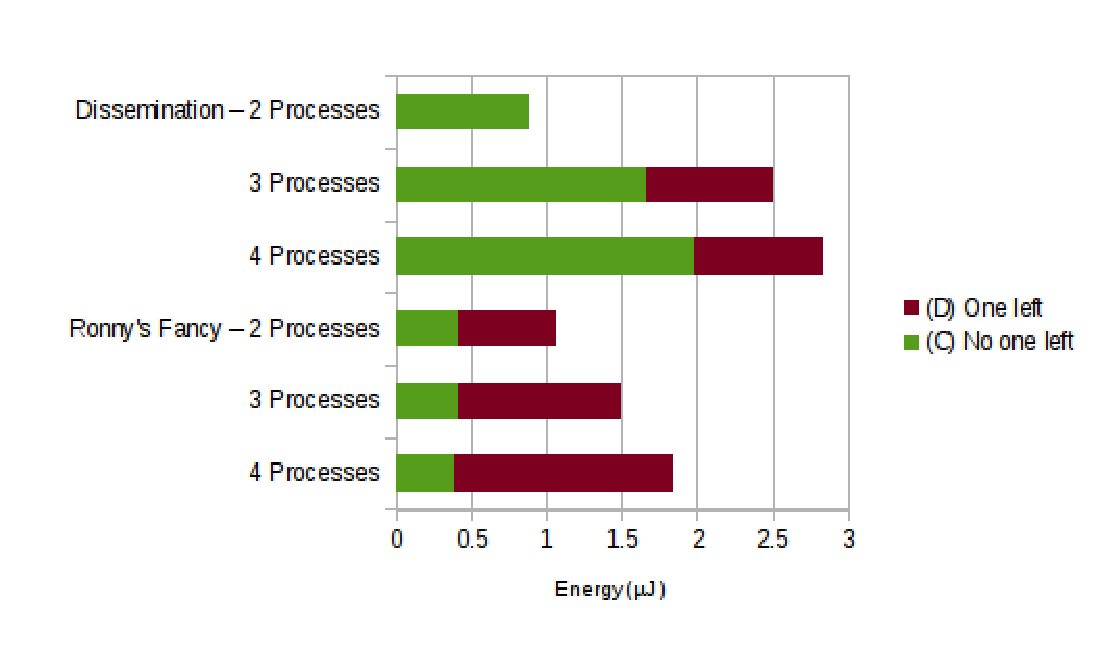
\includegraphics[height=4.3cm]{charts/df-energy-work-1000-partition}
			\end{minipage}
			\caption{Distribution of total time spent and energy consumed}
			\label{fig:df-work-1000-partition}
		\end{figure}
		\begin{itemize}
			\item excluding (A) and (B) because long.
			\item first one to leave for rf unrealistic as in Figure~\ref{fig:df-work-100-partition}
		\end{itemize}
	\item Dissemination: distribution of total time spent and energy consumed: Figure~\ref{fig:d-work-1000-partition}
		\begin{figure}[htbp]
			\centering
			\begin{minipage}{0.43\linewidth}
				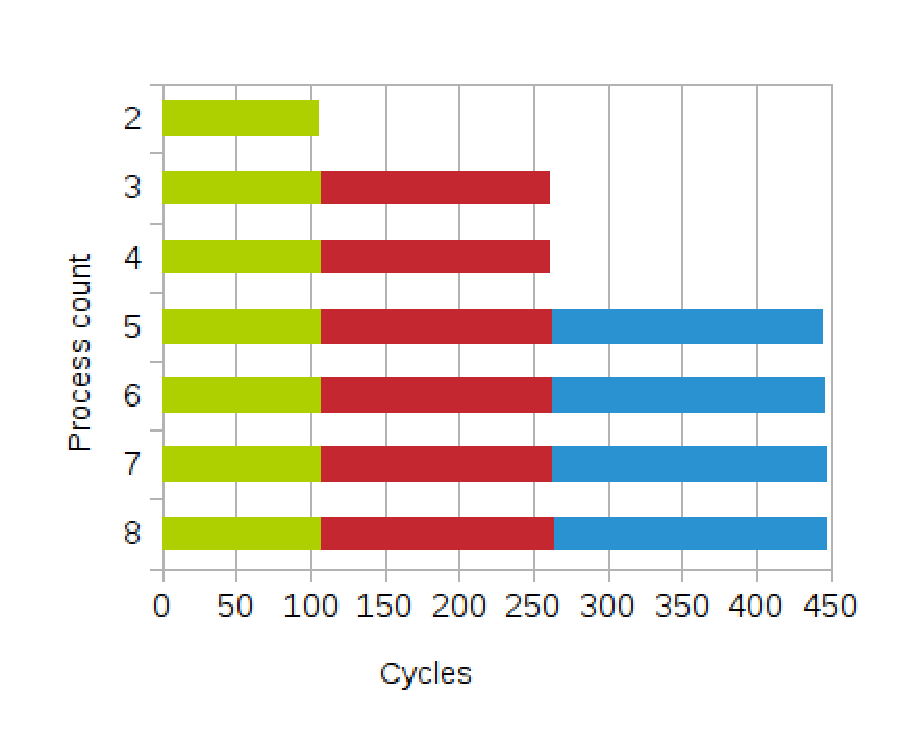
\includegraphics[height=4.2cm]{charts/d-time-work-1000-partition}
			\end{minipage}
			\begin{minipage}{0.56\linewidth}
				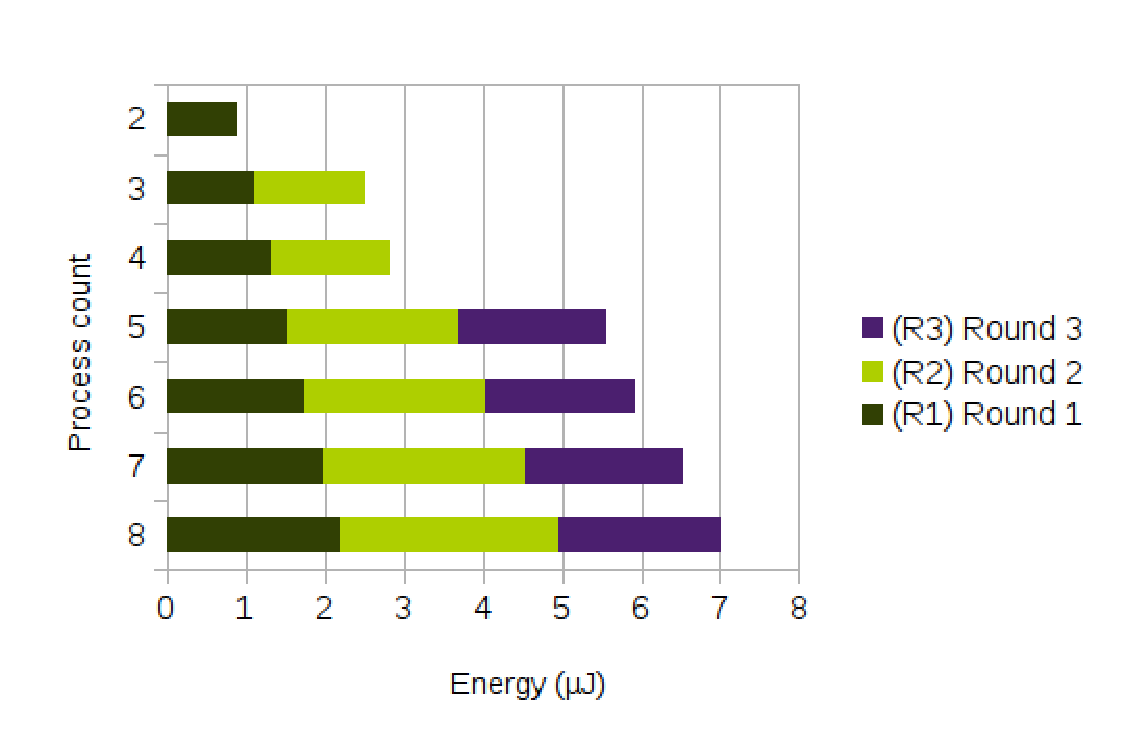
\includegraphics[height=4.2cm]{charts/d-energy-work-1000-partition}
			\end{minipage}
			\caption{Distribution of total time spent and energy consumed for the Dissemination Barrier}
			\label{fig:d-work-1000-partition}
		\end{figure}
		\begin{itemize}
			\item as expected
			\item In comparison to Figure~\ref{fig:d-work-100-partition} there is almost no additional time cost per process associated. CTMC semantic effect diminishes because the remote writes in the rounds are approximately serial. Therefore a write is oftentimes activatable at the same time as other processes are repeatedly executing local reads. The expected time such a write takes is then $\approx 100$ CPU cycles.
			\item the durations for the rounds are related to the progress explanation in Section~\ref{sssec:analysis-general-distributed}. When the last process arrives at the barrier, exactly one remote write is needed to finish round one, two more writes are needed to finish round two and four writes are needed to finish the third round. Therefore, and because of CTMC interleaving semantics, approximately 100, 150 and 183 cycles are needed to finish rounds one, two and three.
			\item Energy usage increases with each additional progress for the same reasons as in Figure~\ref{fig:d-work-100-partition}
			\item progress problem.
			\item there is a fixed cost for each additional round in the Dissemination Barrier.
			\item due to model checking limitations (a very large state space), we cannot quantify beyond four processes, i.e. two rounds.
			\item as shown in Figure~\ref{fig:d-work-1000-partition} ronny's fancy is indeed quicker.
			\item in relation to the results from work period 100, ronny's fancy could not increase its headway at work period 1000.
			\item this does not necessarily mean that the progress problem does not exist. It might for example mean that ronny's fancy does not handle this situation as efficiently as we expected or that it did better than we expected for the 100 cycle work period case. Either way it is definitely possible to be generally faster than the Dissemination Barrier is for this scenario.
		\end{itemize}
	\item rate of power consumption per phase: Figure~\ref{fig:df-power-work-1000}
		\begin{figure}[htbp]
			\centering
			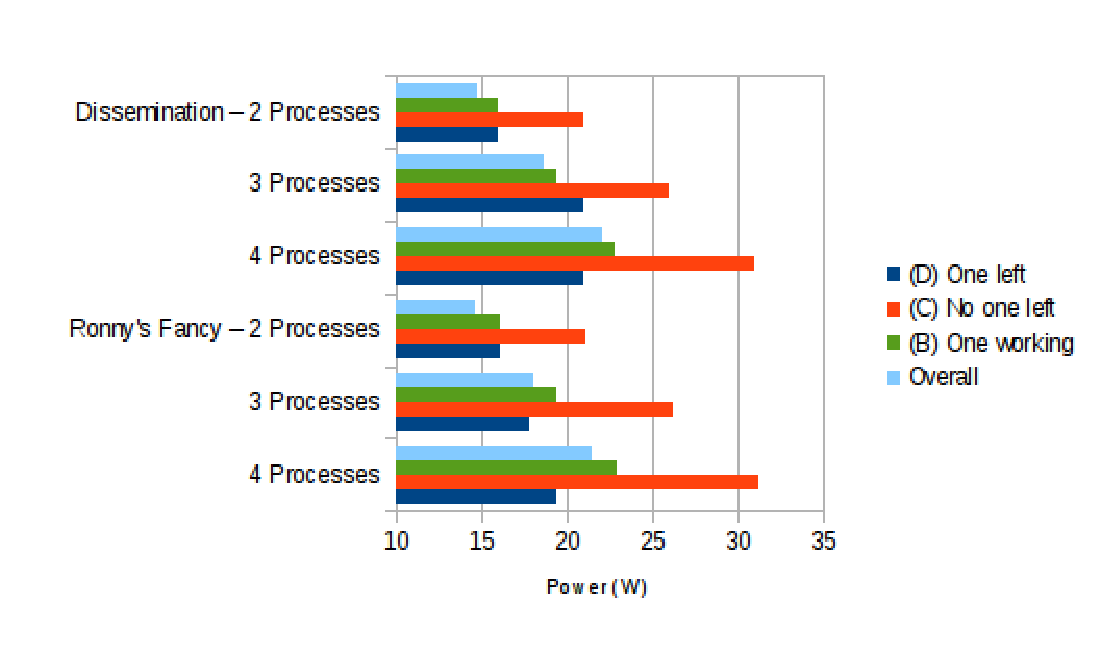
\includegraphics[width=10cm]{charts/df-power-work-1000}
			\caption{Rate of energy consumption for each phase}
			\label{fig:df-power-work-1000}
		\end{figure}
		\begin{itemize}
			\item overall power consumption slightly lower because of the 1000 cycle work period.
			\item everything else similar to Figure~\ref{fig:df-power-work-100}.
		\end{itemize}
	\item number of remote transfers
		\begin{itemize}
			\item remote transfer is a generic term including remote reads and remote writes.
			\item fixed for Dissemination as explained in Section~\ref{sssec:analysis-general-distributed}. $n \cdot \lceil \log _2~n \rceil$
			\item number of successful transfers (transfers that read from an arrived processes) between $2 \cdot (n-1)$ and $n \cdot (n-1)$. Both practically never happen because randomness and access pattern.
			\item failed transfers (transfers where you read from a not yet arrived process).
			\item hard to estimate, because the randomness of the system defines this number.
			\item work=100. Figure~\ref{tab:df-transfers-100}
				\begin{table}[htbp]
					\centering
					\caption{Expected number of remote transfers}
					\vspace{0.2cm}
					\begin{tabular}{r | r | r r}
						              & Threads & Successful transfers & Failed transfers \\
						\hline
						Dissemination & 2       & 2                     &                 \\
						              & 3       & 6                     &                 \\
						              & 4       & 8                     &                 \\
						\hline
						Ronny's Fancy & 2       & 2                     & 0.99            \\
						              & 3       & 4.74                  & 1.73            \\
						              & 4       & 7.98                  & 2.44            \\
					\end{tabular}
					\label{tab:df-transfers-100}
				\end{table}
				\begin{itemize}
					\item as expected ronny's fancy issues more remote transactions than the Dissemination Barrier.
					\item it is still relatively low.
					\item especially the number of failed remote accesses is low in comparison to the number of successful ones.
					\item For process count 5, and other non-power of two process counts the situation might turn out better for ronny's fancy, because of the additional rounds and thus additional transfers needed.
				\end{itemize}
			\item work=1000. Table~\ref{tab:df-transfers-1000}
				\begin{table}[htbp]
					\centering
					\caption{Expected number of remote transfers}
					\vspace{0.2cm}
					\begin{tabular}{r | r r}
						Threads & Successful transfers & Failed transfers \\
						\hline
						2       & 2                     & 9.9             \\
						3       & 4.95                  & 22.89           \\
						4       & 8.78                  & 38.05           \\
					\end{tabular}
					\label{tab:df-transfers-1000}
				\end{table}
				\begin{itemize}
					\item number of successful transfers very similar to work=100.
					\item failed transfers is of course more than before since ronny's fancy is busy waiting on remote memory.
					\item back-off strategies could be used, if one would want to save the lost bandwidth, latency and energy in exchange for a longer duration of the protocol.
				\end{itemize}
		\end{itemize}
\end{itemize}

%%%%%%%%%%%%%%%%%%%%%%%%%%%%%%%%%%%%%%%
\subsection{Discussion}
\label{ssec:analysis-discussion}
\begin{itemize}
	\item meta
		\begin{itemize}
			\item maybe leave out and put it in the evaluation section. If you have something to sum up or perhaps compare measurement and model checking then this section might still be useful.
			\item reread \url{http://www.usca.edu/biogeo/researchguide/writing.html#Results}
			\item "Discuss and explain your results"
			\item "Show how they support your thesis (or, if they don't, come up with a damned good reason real quick)"
			\item "It is important to separate objective facts clearly from their discussion"
		\end{itemize}

	\item all analysed barriers are functionally correct in the sense that they indeed perform a barrier synchronization.
	\item all shown barriers finish reasonably quick.
	\item all considered barriers use a reasonable amount of energy.

	\item shared memory
	\item despite atomic operations the Central Counter barrier is quick.
	\item ronny's simple approach to trade less time writing for more time reading does not pay off. Because: (1) in a balanced scenario the time lost due to queuing atomic operations is small. (2) no atomic operations means more busy waiting, thus more energy used.
	\item ronny's simple performs worse in all considered scenarios.

	\item distributed memory
	\item ronny's fancy barrier issues not much more remote operations than the Dissemination barrier despite busy waiting on remote memory.
	\item as conjectured in Section~\ref{sssec:analysis-general-distributed} the Dissemination barrier wastes substantial time when processes arrive even in small intervals.
	\item for non-power of two process counts the Dissemination barrier wastes substantial time and energy due to its $\lceil \log_2 n \rceil$ number of rounds and $n \cdot \lceil \log_2 n \rceil$ number of remote operations.
	\item ronny's fancy outperforms the Dissemination barrier in all scenarios.

	\item CTMC model checking semantic for interleaving modules is different from the intuitive notion of parallel execution. Therefore one has to exercise caution when interpreting model checking results.
\end{itemize}

%%%%%%%%%%%%%%%%%%%%%%%%%%%%%%%%%%%%%%%%%%%%%%%%%%%%%%%%%%%%%%%%%%%%%%%%%%%%%%%
\section{Conclusion and future work}
\label{sec:conclusion}
Conclusion:
\begin{itemize}
	\item meta
		\begin{itemize}
			\item "Don't leave it at the discussion: discuss what you/we can learn from the results. Draw some real conclusions. Separate discussion/interpretation of the results clearly from the conclusions you draw from them"
			\item condense results into a small passage
			\item ?repeat claim - overarching thesis - present an answer?
		\end{itemize}
	\item (overarching (1) barriers can be improved, (2) pW/CS (3) model checking is useful)
	\item we had an in-depth look at how current barriers work, and by which means barriers can be designed.
	\item We presented three new barriers, two of which show promise and we therefore conclude that there exists potential to improve barrier protocols.
	\item To achieve the shown performance, both new barriers do not use a fixed communication pattern, as today's barrier algorithms do, but rely on randomness to yield better results. This is one of the fundamental principles of pW/CS and shows that it is useful.
	\item Model checking enabled us to look into barrier algorithms at a more fine-grained level than measurement-based methods could hope to.
	\item We demonstrated the aptitude of model checking as a method for analysing synchronization protocols and algorithms in general.
\end{itemize}

Future work:
\begin{itemize}
	\item meta
		\begin{itemize}
			\item "Identify all shortcomings/limitations of your work, and discuss how they could be fixed"
		\end{itemize}
	\item measurement
		\begin{itemize}
			\item conduct measurements of the shared memory barriers (easy). Preliminary tests show that both ronny's simple and ronny's fancy perform better than model checking analysis suggests.
			\item implement ronny's fancy on RDMA hardware and benchmark against established algorithms
		\end{itemize}
	\item widen focus
		\begin{itemize}
			\item evaluate back-off strategies. (technical possibilities. Strategies like exponential back-off, linear back-off, etc.)
			\item mwait (wait for a change in a variable. Not polling actively).
			\item model and measure dissemination and ronny's fancy for shared memory.
		\end{itemize}
	\item CTMC exit rate semantic
		\begin{itemize}
			\item why is it like that?
			\item work around it?
			\item attempt to invent an variations on the CTMC semantic to suit modelling parallel execution better?
			\item try alternative model checking formalisms.
		\end{itemize}
	\item modelcheck larger: more threads. Symmetry reduction. Partial order reduction. Manual reduction.
	\item model check more fine-grained
		\begin{itemize}
			\item model multi layered cache. More realistic.
			\item model resource conflict. (We currently assume infinite bandwidth and amount of communication that can take at the same time)
			\item model topology between processes. Like cores/dies/packages/nodes/blades. Because it influence latency.
		\end{itemize}
	\item explore variations of the new barriers
		\begin{itemize}
			\item Ronny's fancy barrier: Try different i increment strategies. Or perhaps randomize the choice of i.
			\item use remote write \& local read instead of local write \& remote read, because remote writing is preferred on some platforms, e.g. on the Epiphany\cite{epiphany}. AND this way one might be able to avoid failed remote operations entirely and keep busy waiting local.
		\end{itemize}
	\item misc
		\begin{itemize}
			\item~
		\end{itemize}
\end{itemize}


%%%%%%%%%%%%%%%%%%%%%%%%%%%%%%%%%%%%%%%%%%%%%%%%%%%%%%%%%%%%%%%%%%%%%%%%%%%%%%%
\appendix

%%%%%%%%%%%%%%%%%%%%%%%%%%%%%%%%%%%%%%%%%%%%%%%%%%%%%%%%%%%%%%%%%%%%%%%%%%%%%%%
\pagebreak
\section{Appendix}
\label{sec:appendix}
\subsection{Energy reference measurement for estimating the model parameters}
The CPU we used is an Intel\textregistered~Core\texttrademark~i5-2520M clocked at 2.50GHz.
\label{ssec:energy-measurement}
\begin{table}[h!]
	\centering
	\caption{Reference measurement (without Hyper-Threading)}
	\vspace{0.2cm}
	\begin{tabular}{r | r | r r r}
		                         & Thread & Time     & Energy    & Rate of      \\
		                         & count  & (Cycles) & consumpt. & energy cons. \\
		                         &        &          & (nJ)      & (W)          \\
		\hline
		Idle                     &        &          &           &  4.0 \\
		Off-core under load      &        &          &           &  6.8 \\
		Load                     & 1      &          &           & 19.6 \\
		                         & 2      &          &           & 28.4 \\
		Busy waiting             & 1      &          &           & 16.4 \\
		                         & 2      &          &           & 22.8 \\
		\hline
		Add\&fetch (contested)   & 2      &    137.6 &     893.7 & 16.2 \\
		Add\&fetch (uncontested) & 2      &     19.3 &     158.5 & 20.5 \\
		Central Counter Barrier  & 2      &    227.4 &    1667.0 & 18.3 \\
		Ronny's simple barrier   & 2      &    114.0 &    1076.1 & 23.6 \\
		Dissemination Barrier    & 2      &    144.0 &    1400.3 & 24.3 \\
		Ronny's fancy barrier    & 2      &     42.1 &     433.4 & 25.7 \\
	\end{tabular}
\end{table}
\begin{table}[h!]
	\centering
	\caption{Reference measurement (with Hyper-Threading)}
	\vspace{0.2cm}
	\begin{tabular}{r | r | r r r}
		                          & Thread & Time     & Energy    & Rate of      \\
		                          & count  & (Cycles) & consumpt. & energy cons. \\
		                          &        &          & (nJ)      & (W)          \\
		\hline
		Idle                      &        &          &           &  4.0 \\
		\arrayrulecolor{lightgray}\hline\arrayrulecolor{black}
		Off-core under load       &        &          &           & 12.6 \\
		\arrayrulecolor{lightgray}\hline\arrayrulecolor{black}
		Load                      & 1      &          &           & 19.6 \\
		                          & 2      &          &           & 19.7 \\
		                          & 3      &          &           & 28.0 \\
		                          & 4      &          &           & 28.3 \\
		\arrayrulecolor{lightgray}\hline\arrayrulecolor{black}
		Busy waiting              & 1      &          &           & 17.2 \\
		                          & 2      &          &           & 17.5 \\
		                          & 3      &          &           & 22.9 \\
		                          & 4      &          &           & 22.9 \\
		\hline
		Add\&fetch (contested)    & 2      &    122.2 &     700.2 & 14.3 \\
		                          & 3      &    136.6 &     903.3 & 16.5 \\
		                          & 4      &    354.6 &    2349.9 & 16.7 \\
		\arrayrulecolor{lightgray}\hline\arrayrulecolor{black}
		Add\&fetch (unconstested) & 2      &     45.2 &     283.8 & 15.7 \\
		                          & 3      &     46.9 &     389.0 & 20.7 \\
		                          & 4      &     47.5 &     396.6 & 20.9 \\
		\arrayrulecolor{lightgray}\hline\arrayrulecolor{black}
		Central Counter Barrier   & 2      &     86.5 &     647.1 & 18.7 \\
		                          & 3      &    314.0 &    2613.6 & 20.8 \\
		                          & 3      &    442.8 &    3908.3 & 22.0 \\
		\arrayrulecolor{lightgray}\hline\arrayrulecolor{black}
		Ronny's simple barrier    & 2      &     45.4 &     359.2 & 19.8 \\
		                          & 3      &    157.8 &    1614.5 & 25.6 \\
		                          & 4      &    198.3 &    2174.1 & 27.4 \\
		\arrayrulecolor{lightgray}\hline\arrayrulecolor{black}
		Dissemination Barrier     & 2      &     94.4 &     785.3 & 20.8 \\
		                          & 3      &    297.4 &    3189.0 & 26.8 \\
		                          & 4      &    337.1 &    3960.3 & 29.4 \\
		\arrayrulecolor{lightgray}\hline\arrayrulecolor{black}
		Ronny's fancy barrier     & 2      &     34.3 &     285.9 & 20.8 \\
		                          & 3      &    109.1 &    1205.6 & 27.6 \\
		                          & 4      &    112.1 &    1297.0 & 28.9 \\
	\end{tabular}
\end{table}

\clearpage
\subsection{Raw data of behind figures}
\begin{itemize}
	\item \todo
\end{itemize}

%%%%%%%%%%%%%%%%%%%%%%%%%%%%%%%%%%%%%%%%%%%%%%%%%%%%%%%%%%%%%%%%%%%%%%%%%%%%%%%
\pagebreak
\section{Bibliography}
\label{sec:bibliography}
\renewcommand\refname{\vskip -1cm} %TODO fine tune perhaps
\nocite{*} % insert not cited references
\bibliographystyle{abbrv}
\bibliography{bibliography}{}

\end{document}
